% !TEX program = pdflatex
\documentclass[11pt,a4paper]{article}

\usepackage[a4paper,margin=25mm]{geometry}
\usepackage{graphicx}
\usepackage{booktabs}
\usepackage{siunitx}
\usepackage{amsmath}
\usepackage{float}
\usepackage{caption}
\usepackage{hyperref}
\usepackage{doi}

\title{UV-Induced Extracellular Electrical Responses of Mycelium\\
\large Exploratory Analysis of Static Loading Effects}
\author{}
\date{\today}

\begin{document}
\maketitle

\begin{abstract}
This report documents a reproducible exploratory analysis of extracellular
voltage recordings from mycelium samples subjected to repeated UV
illumination, with and without an additional static load. Three mycelium
recordings were analysed: one without static loading and two independent
recordings with the same nominal static load. An agar control recording was
also examined. The analysis follows the acquisition and filtering procedure
used in the student's original code, but introduces cycle-aligned,
baseline-subtracted response measures and model-independent kinetic
descriptors. The results are treated as pilot observations because repeated
UV cycles within one recording are not independent biological replicates.
\end{abstract}

\section{Experimental data and protocol}

The available datasets are:
\begin{itemize}
    \item \texttt{mycelium\_ch1.npy}: no static weight;
    \item \texttt{mycelium\_ch1\_weight.npy}: static weight, replicate 1;
    \item \texttt{mycelium\_ch1\_weight2.npy}: the same nominal static weight,
          replicate 2;
    \item \texttt{agar\_control\_ch3.npy}: agar control.
\end{itemize}

The acquisition sampling rate is \SI{100}{Hz}. The first UV exposure starts
at \SI{90}{s}, with \SI{60}{s} of UV illumination followed by a nominal
\SI{180}{s} recovery period. This sequence is repeated for 30 UV exposures.

\begin{figure}[H]
\centering
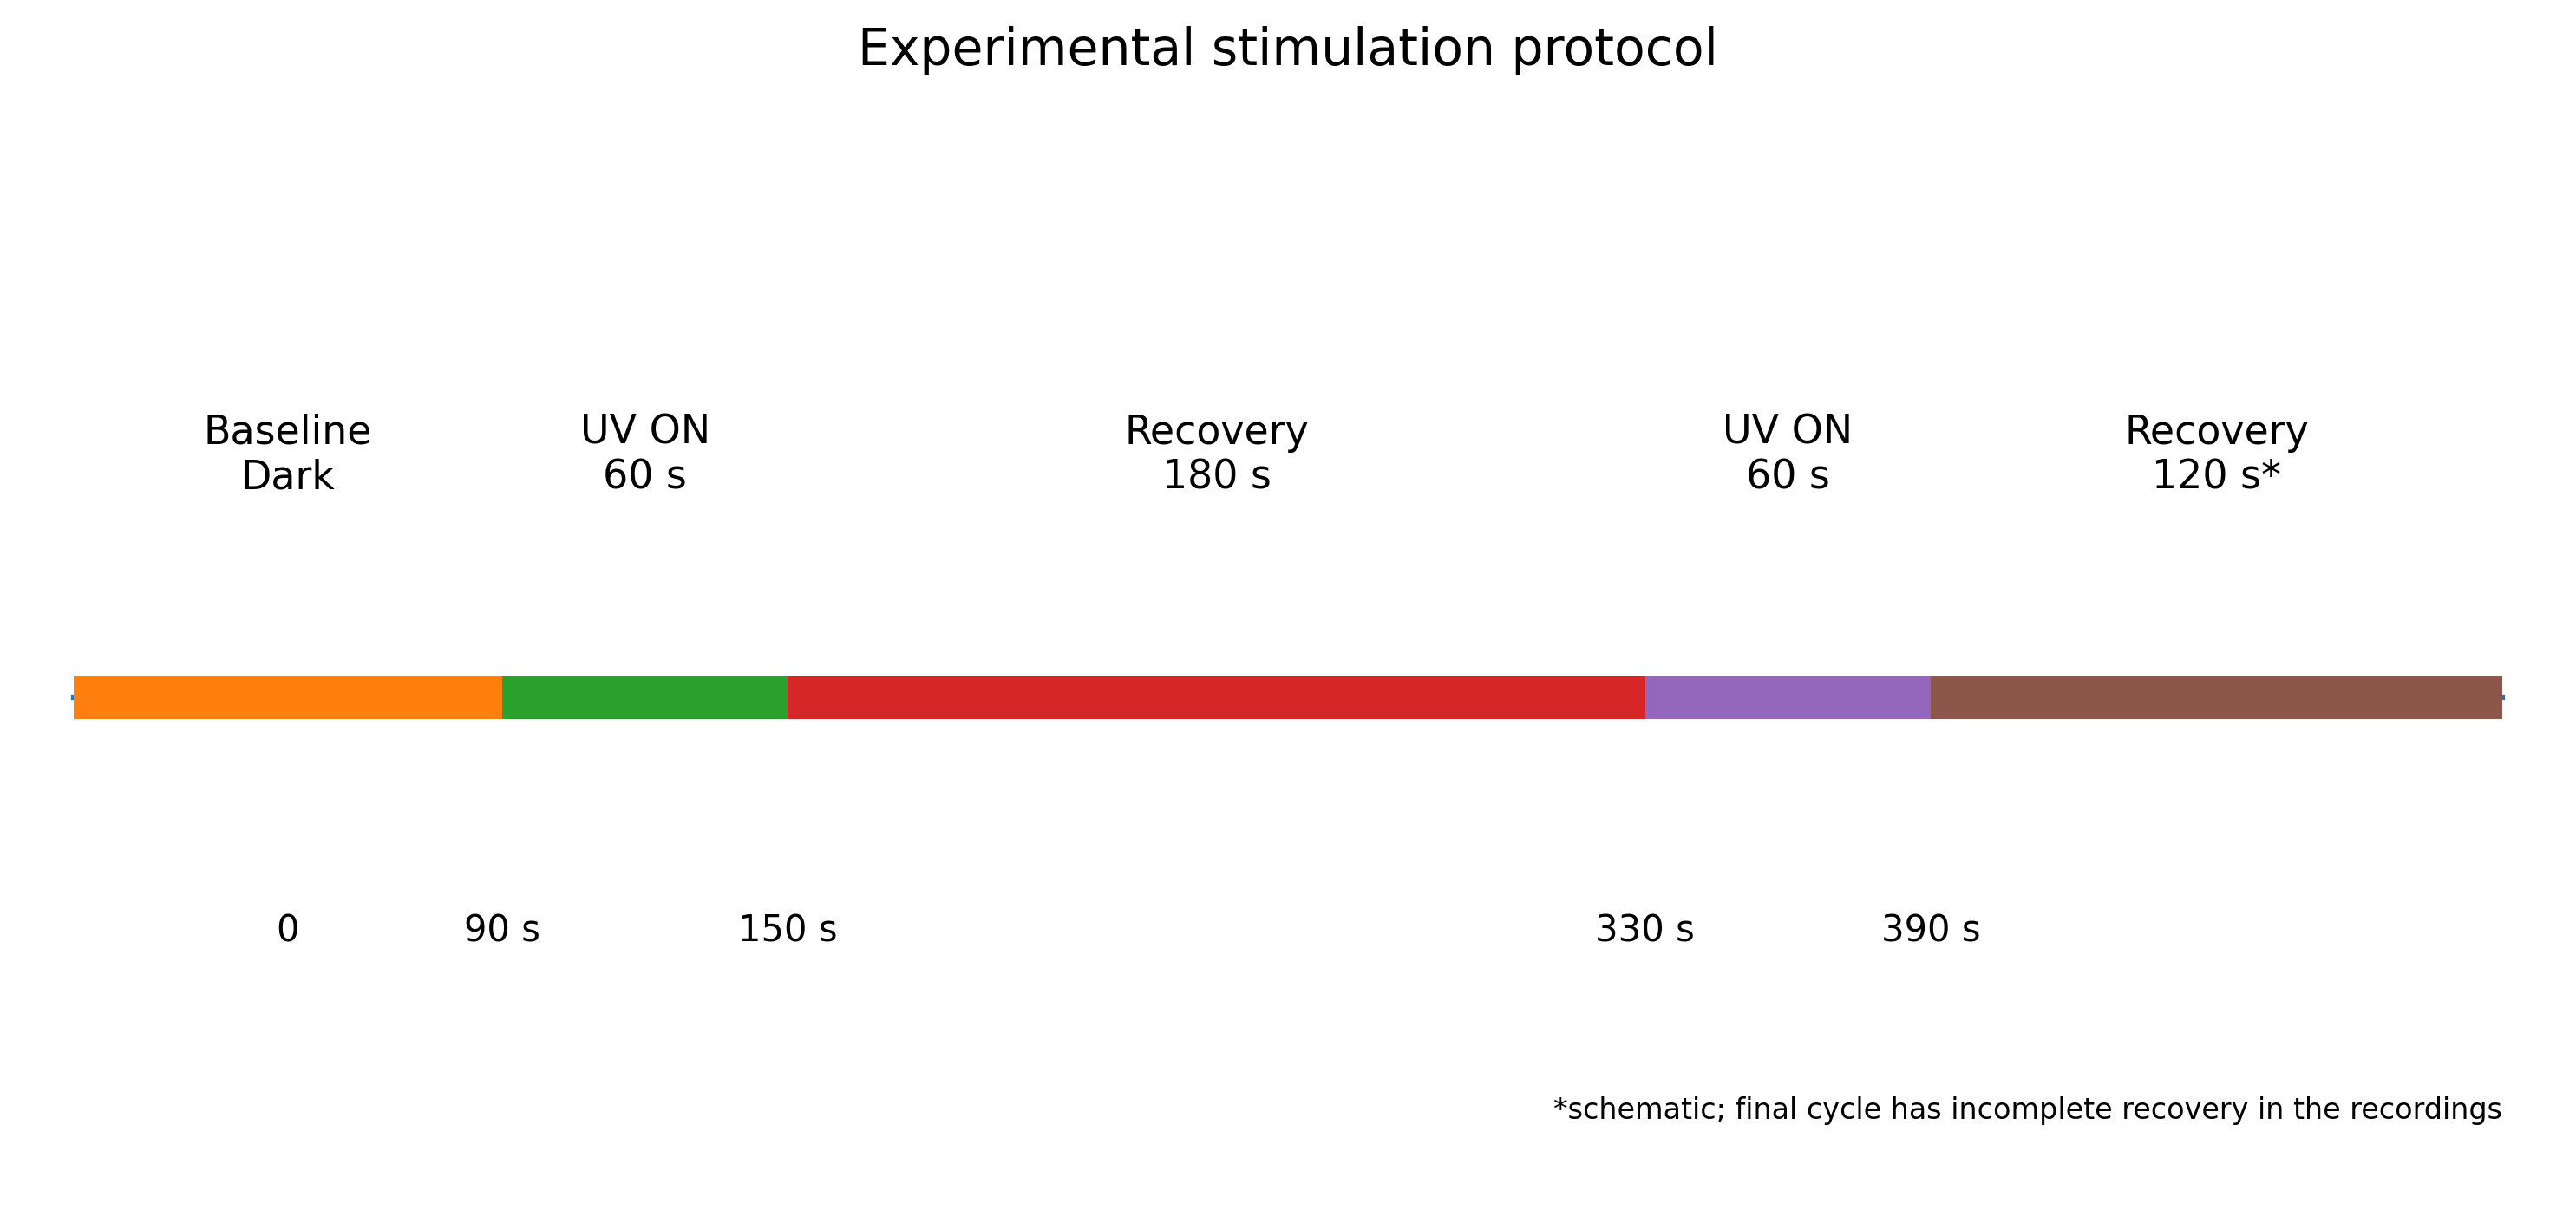
\includegraphics[width=0.95\textwidth]{figures/Figure_1_experimental_protocol.png}
\caption{Schematic of the UV stimulation protocol used for cycle alignment.}
\label{fig:protocol}
\end{figure}

\section{Signal processing}

The stored voltage is converted from volts to millivolts. For consistency
with the student's original analysis, a Savitzky--Golay filter with a
101-sample window and third-order polynomial is applied. At \SI{100}{Hz},
the filtering window corresponds to approximately \SI{1.01}{s}.

Each UV cycle is aligned at UV activation. The preceding \SI{30}{s} is used
as a local baseline, and its median value is subtracted from the complete
cycle. This removes experiment-specific DC offsets and makes the comparison
focus on the UV-induced change.

For the 29 cycles for which the complete \SI{180}{s} recovery interval is
available, the following quantities are calculated:

\begin{align}
A_{\max} &=
\max_{0\le t < 60\,\mathrm{s}}\Delta V(t),\\
t_{50} &: \text{time after the early minimum to reach 50\% of the rise}\\
t_{1/2,\mathrm{rec}} &: \text{time after UV OFF to reach half the
voltage measured immediately before UV OFF},\\
\mathrm{AUC}_{UV} &=
\int_0^{60\,\mathrm{s}}\Delta V(t)\,dt.
\end{align}

The refined $t_{50}$ definition is intentionally model-independent. For
biphasic responses, the early minimum is first identified in the first
\SI{20}{s}; the target is then defined as halfway between this minimum and
the median voltage during the final \SI{10}{s} of UV exposure.

The final UV cycle is omitted from analyses requiring a full recovery
interval because the recording does not contain the complete recovery
period.

\section{Cycle-aligned response}

Figure~\ref{fig:aligned} shows the median cycle-aligned response for the
three mycelium conditions together with the agar control. The shaded regions
around the mycelium curves represent the interquartile range across UV
cycles.

\begin{figure}[H]
\centering
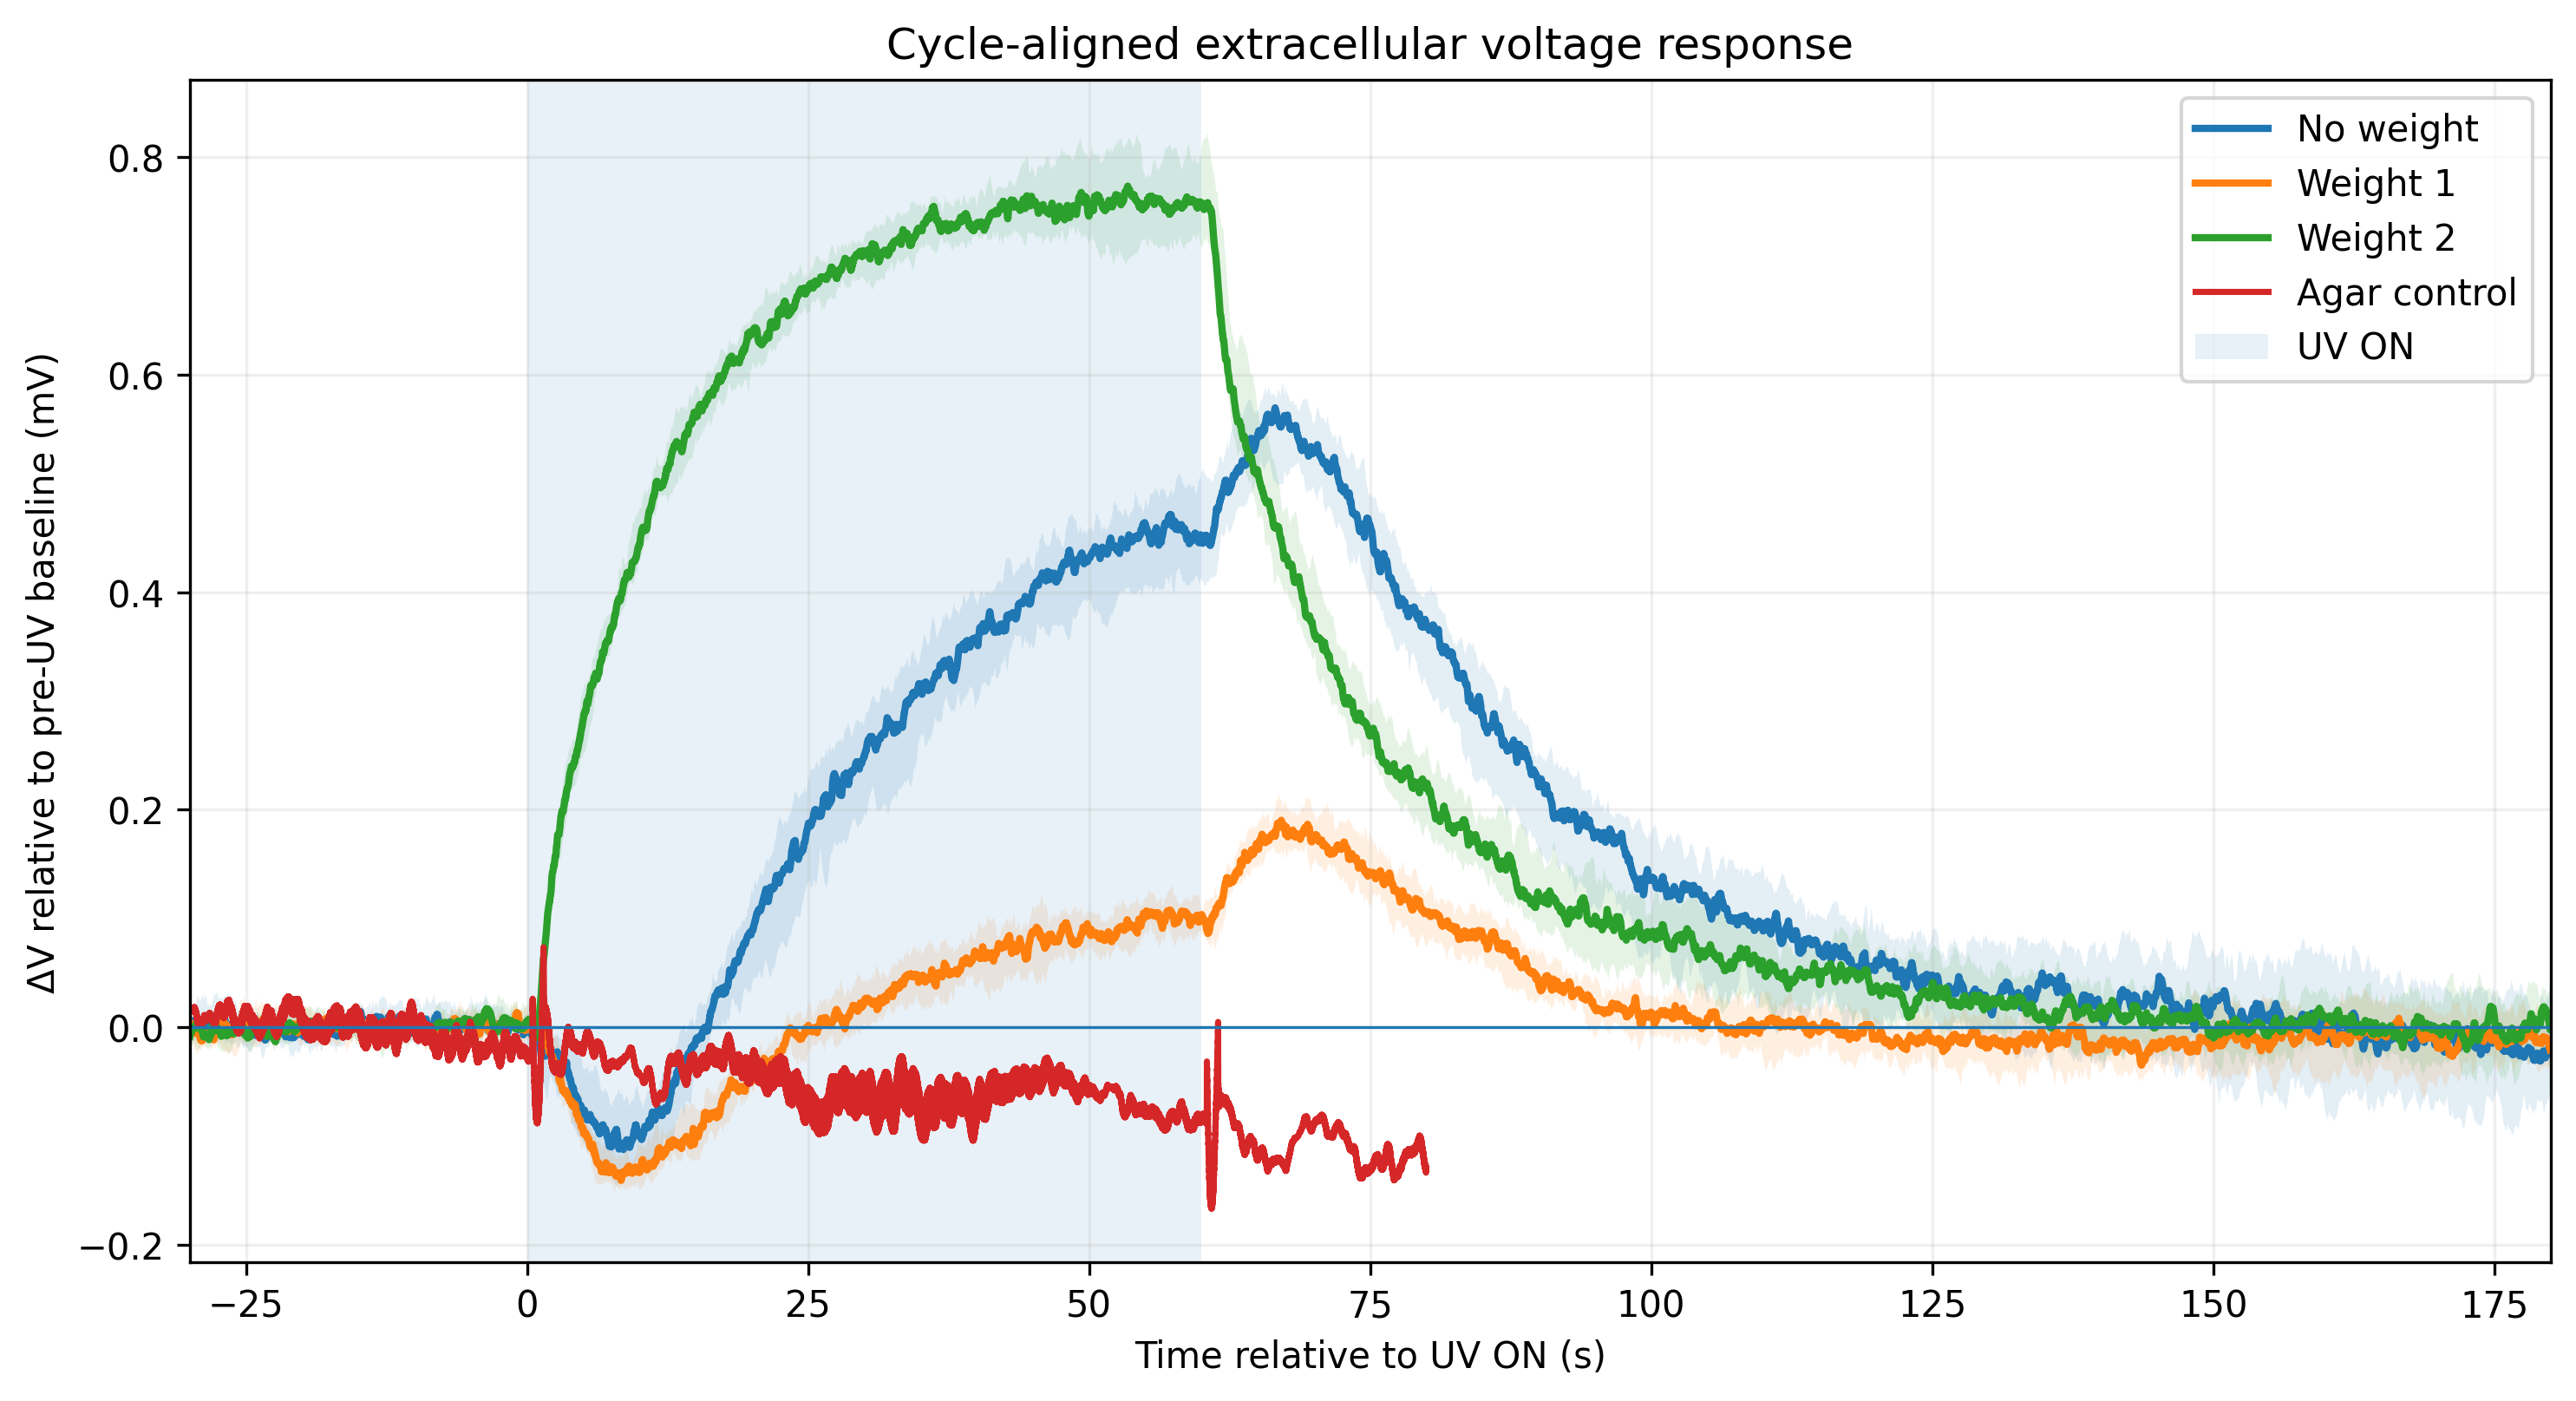
\includegraphics[width=\textwidth]{figures/Figure_2_cycle_aligned_response.png}
\caption{Cycle-aligned extracellular voltage response. Each mycelium curve
is the median across available UV cycles; the shaded region is the
25th--75th percentile range. The agar control is shown as a reference
waveform.}
\label{fig:aligned}
\end{figure}

The recordings exhibit qualitatively different temporal response shapes.
The unloaded and first loaded recordings show an initial negative excursion
followed by a slower positive response. The second loaded recording shows a
predominantly positive response with a substantially faster rise.

The agar control does not reproduce the characteristic sustained positive
response observed in the second loaded mycelium recording. Because the agar
recording is much shorter than the mycelium recordings, it is treated as a
control/reference waveform rather than as a signal to be subtracted from
the mycelium measurements.

\section{Cycle-to-cycle response}

The response amplitude, refined response time, recovery half-time, and
integrated UV response are shown in Figures~\ref{fig:amax}--\ref{fig:auc}.

\begin{figure}[H]
\centering
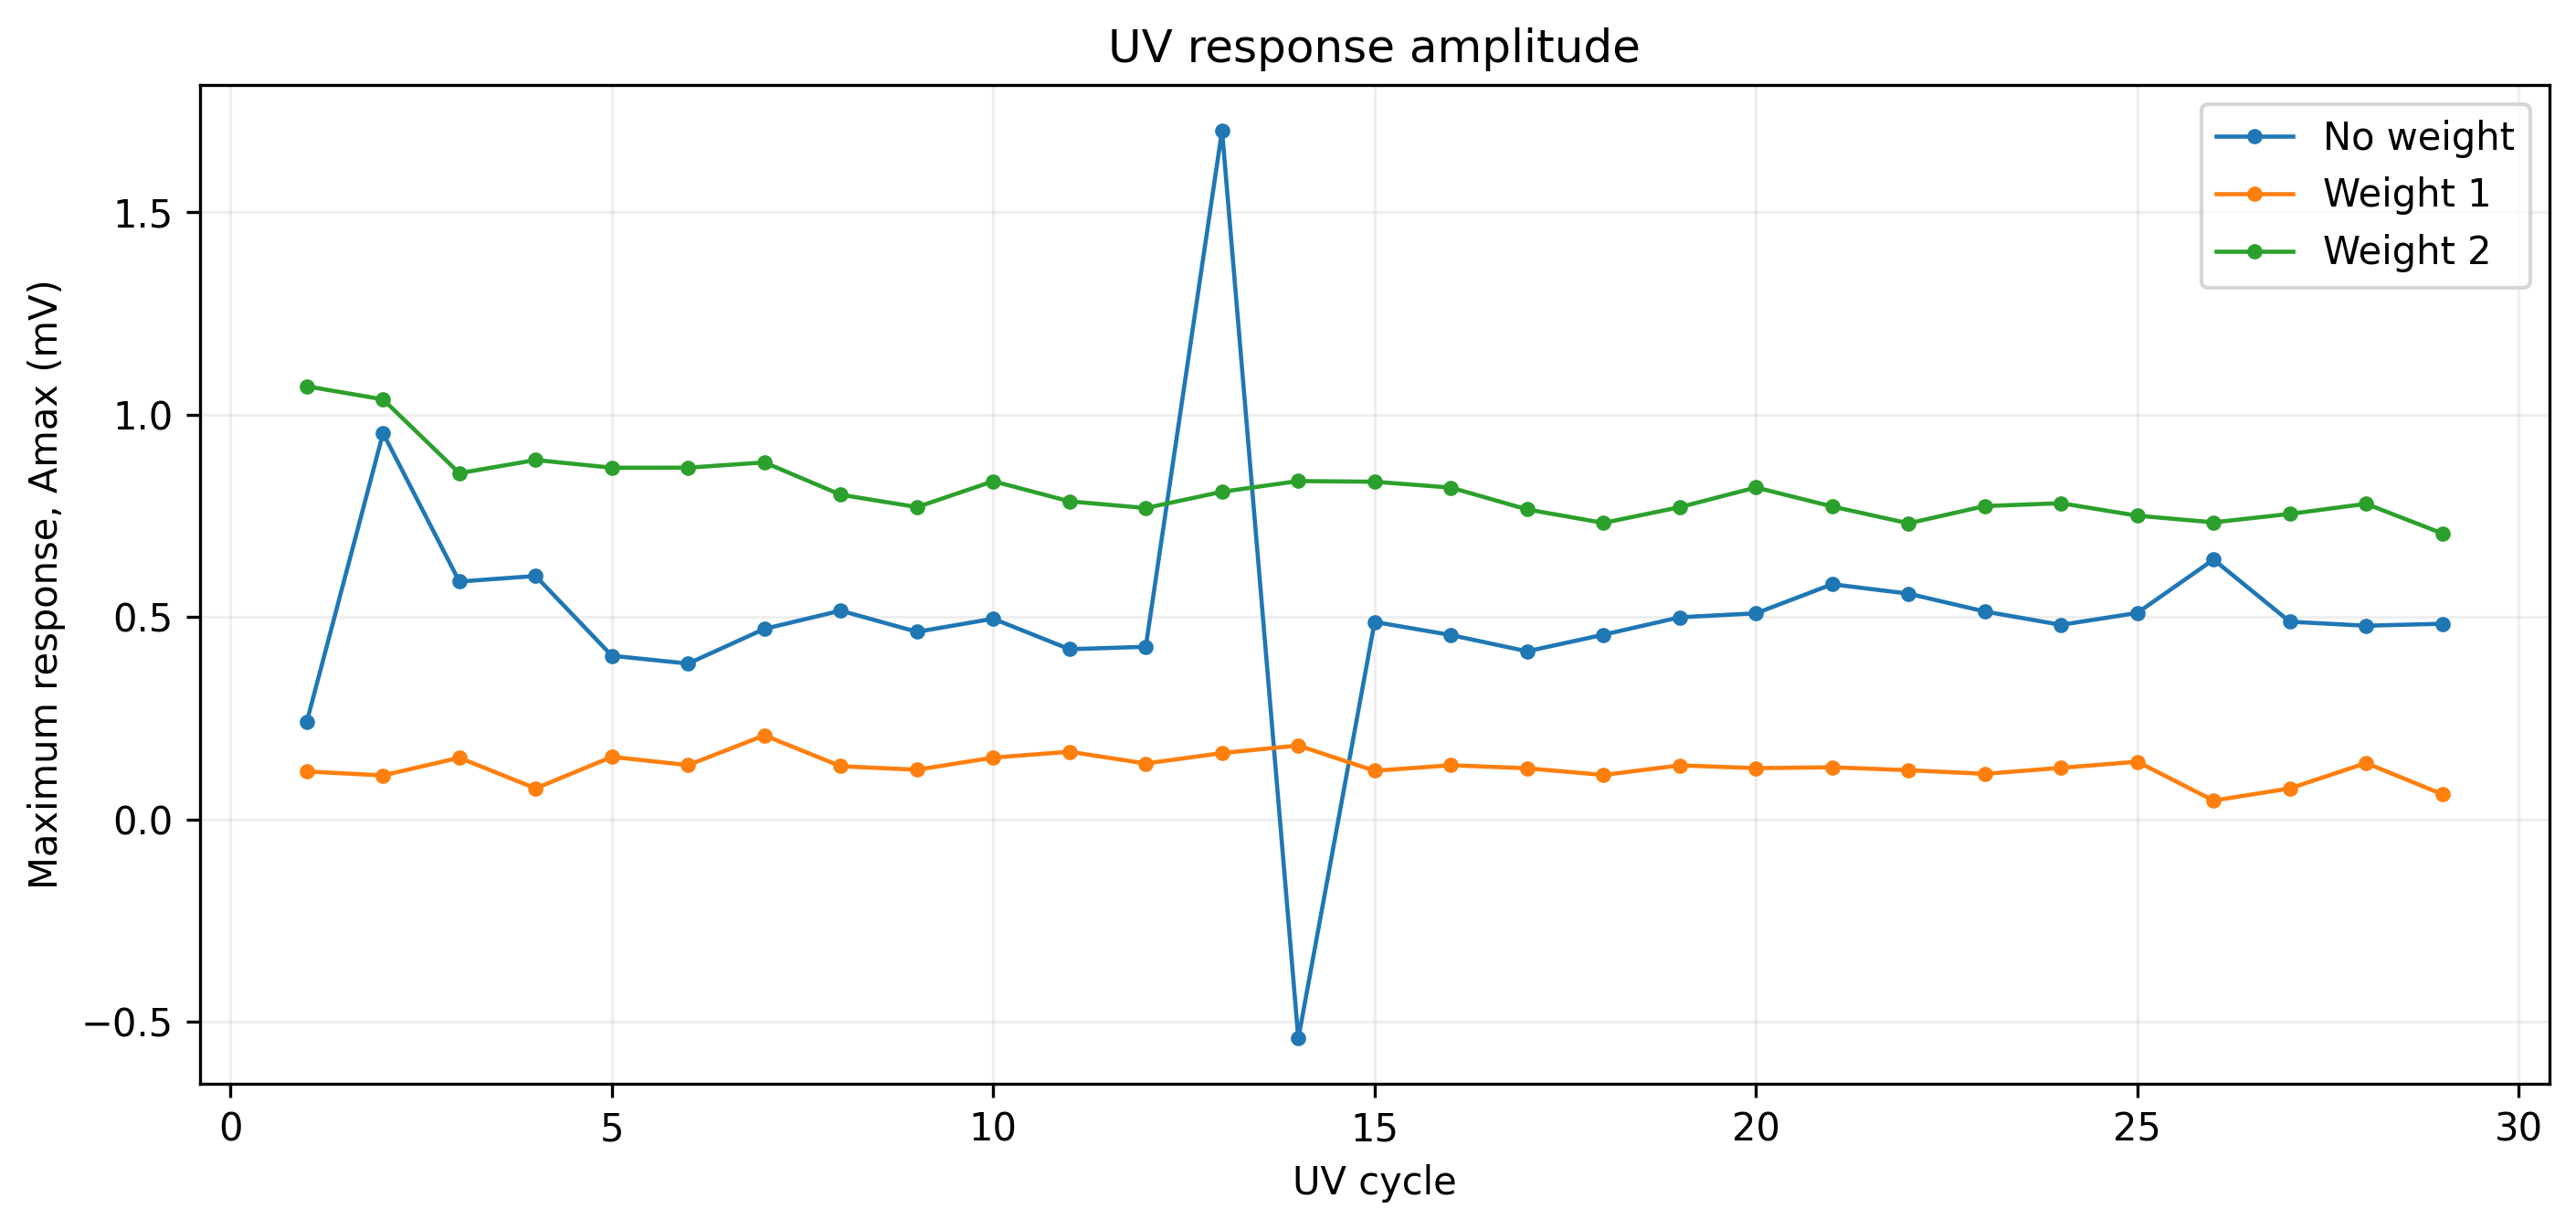
\includegraphics[width=\textwidth]{figures/Figure_3_Amax_mV.png}
\caption{Maximum UV response amplitude for individual UV cycles.}
\label{fig:amax}
\end{figure}

\begin{figure}[H]
\centering
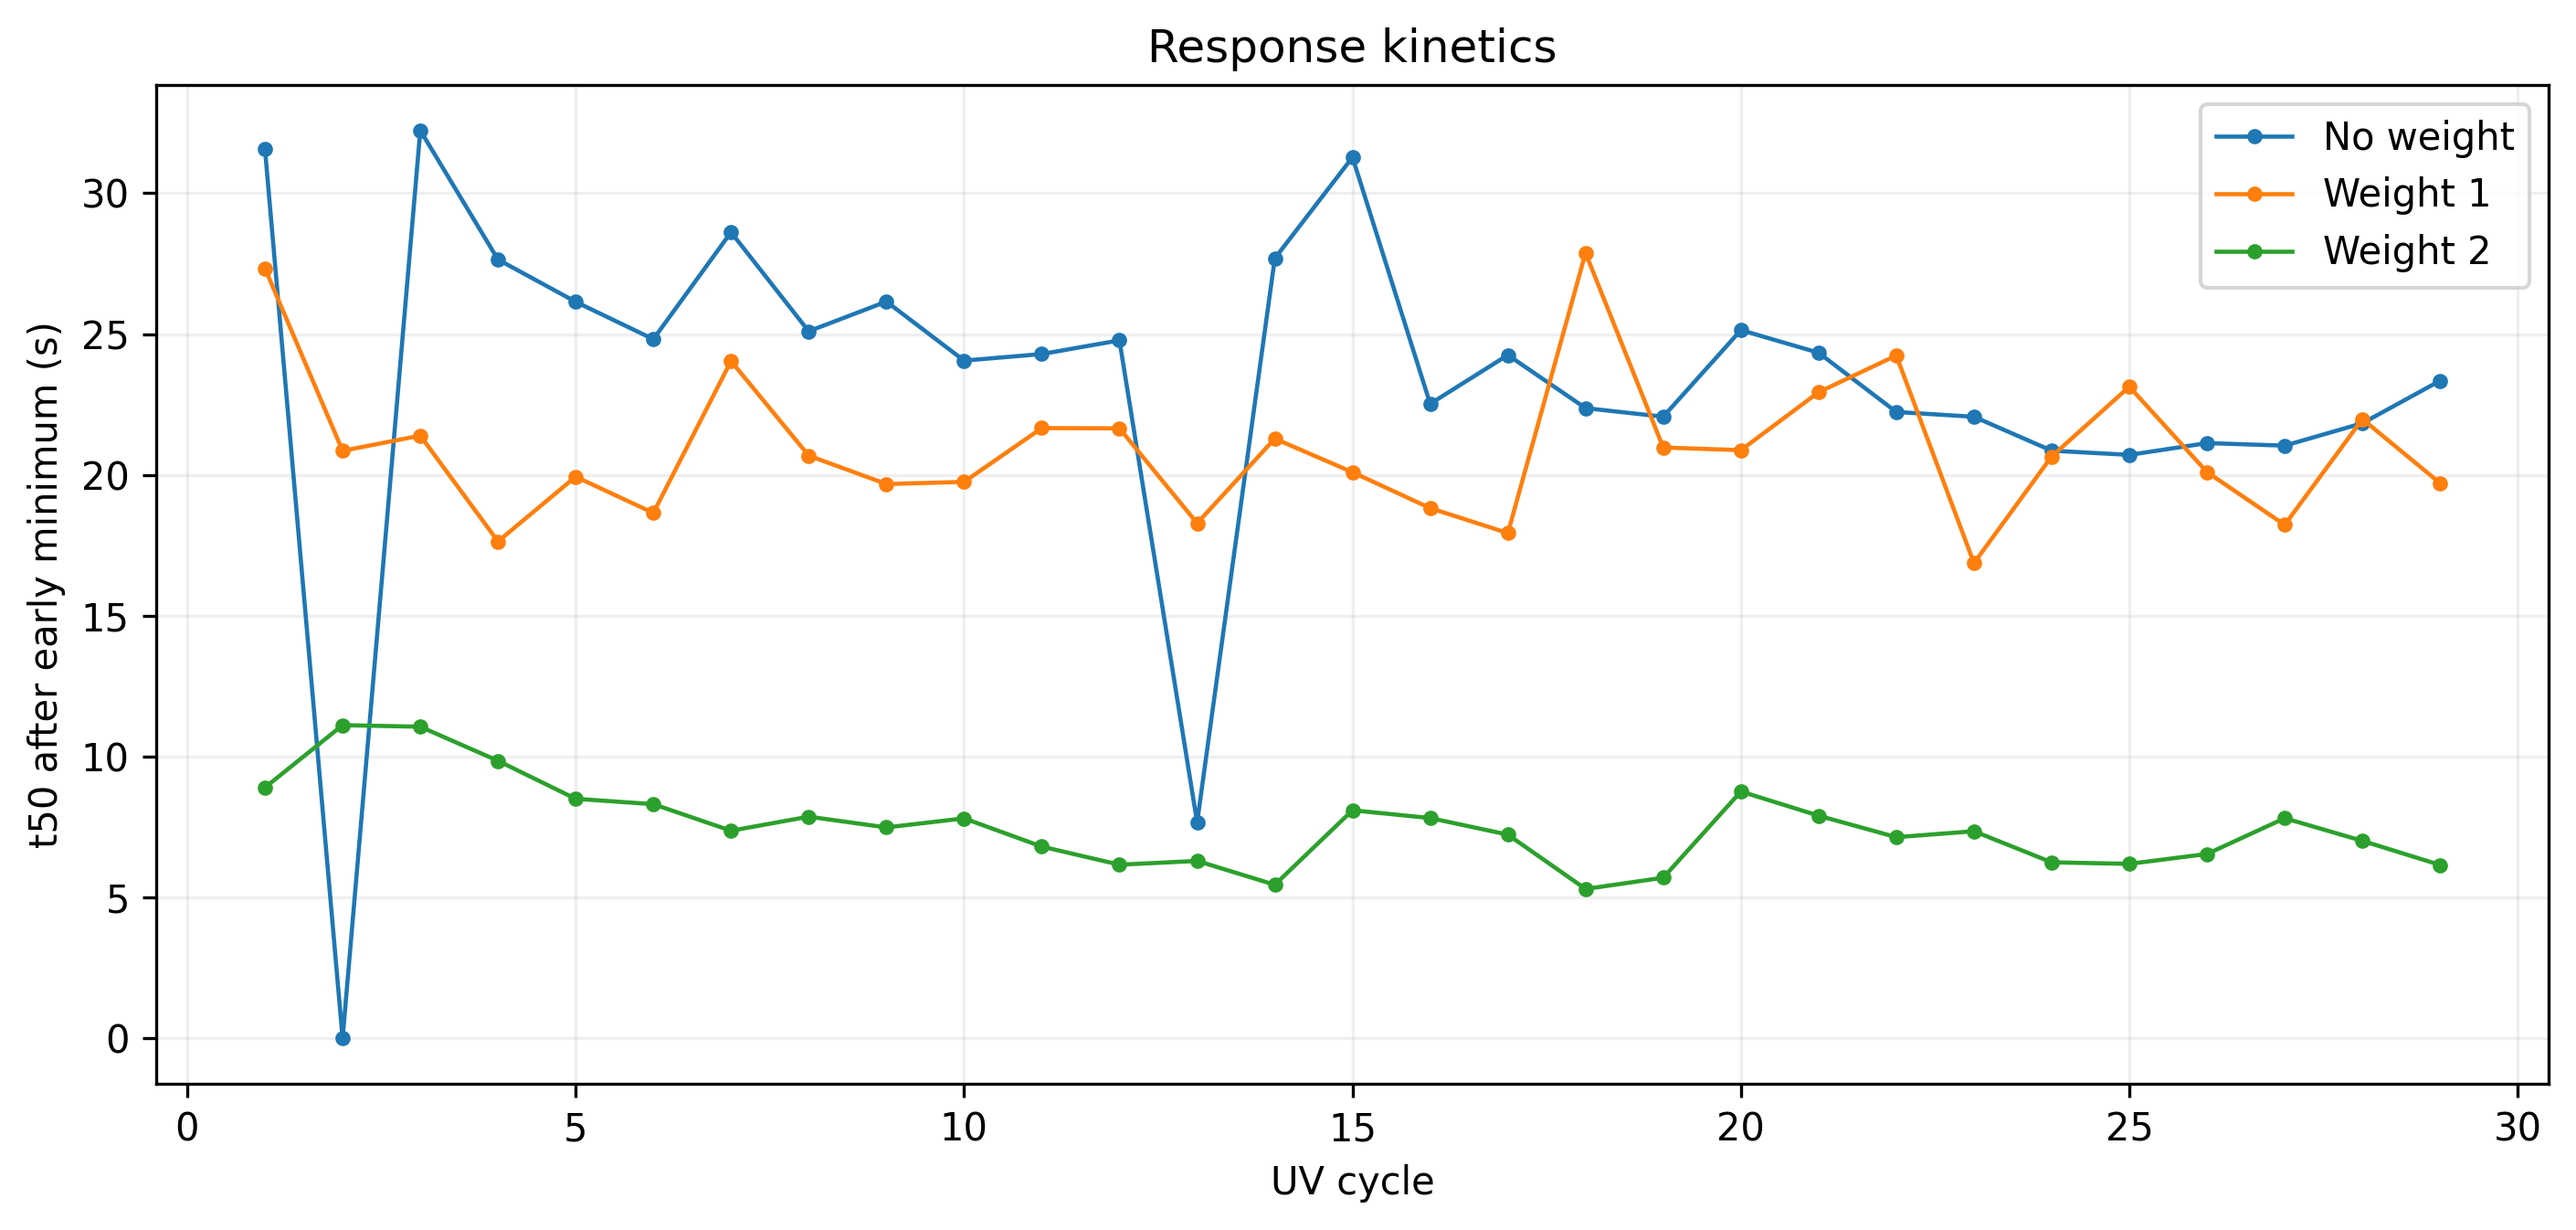
\includegraphics[width=\textwidth]{figures/Figure_3_t50_refined_s.png}
\caption{Refined $t_{50}$ for individual UV cycles. The definition is based
on the early minimum and the sustained UV response, avoiding a forced
single-exponential model for biphasic responses.}
\label{fig:t50}
\end{figure}

\begin{figure}[H]
\centering
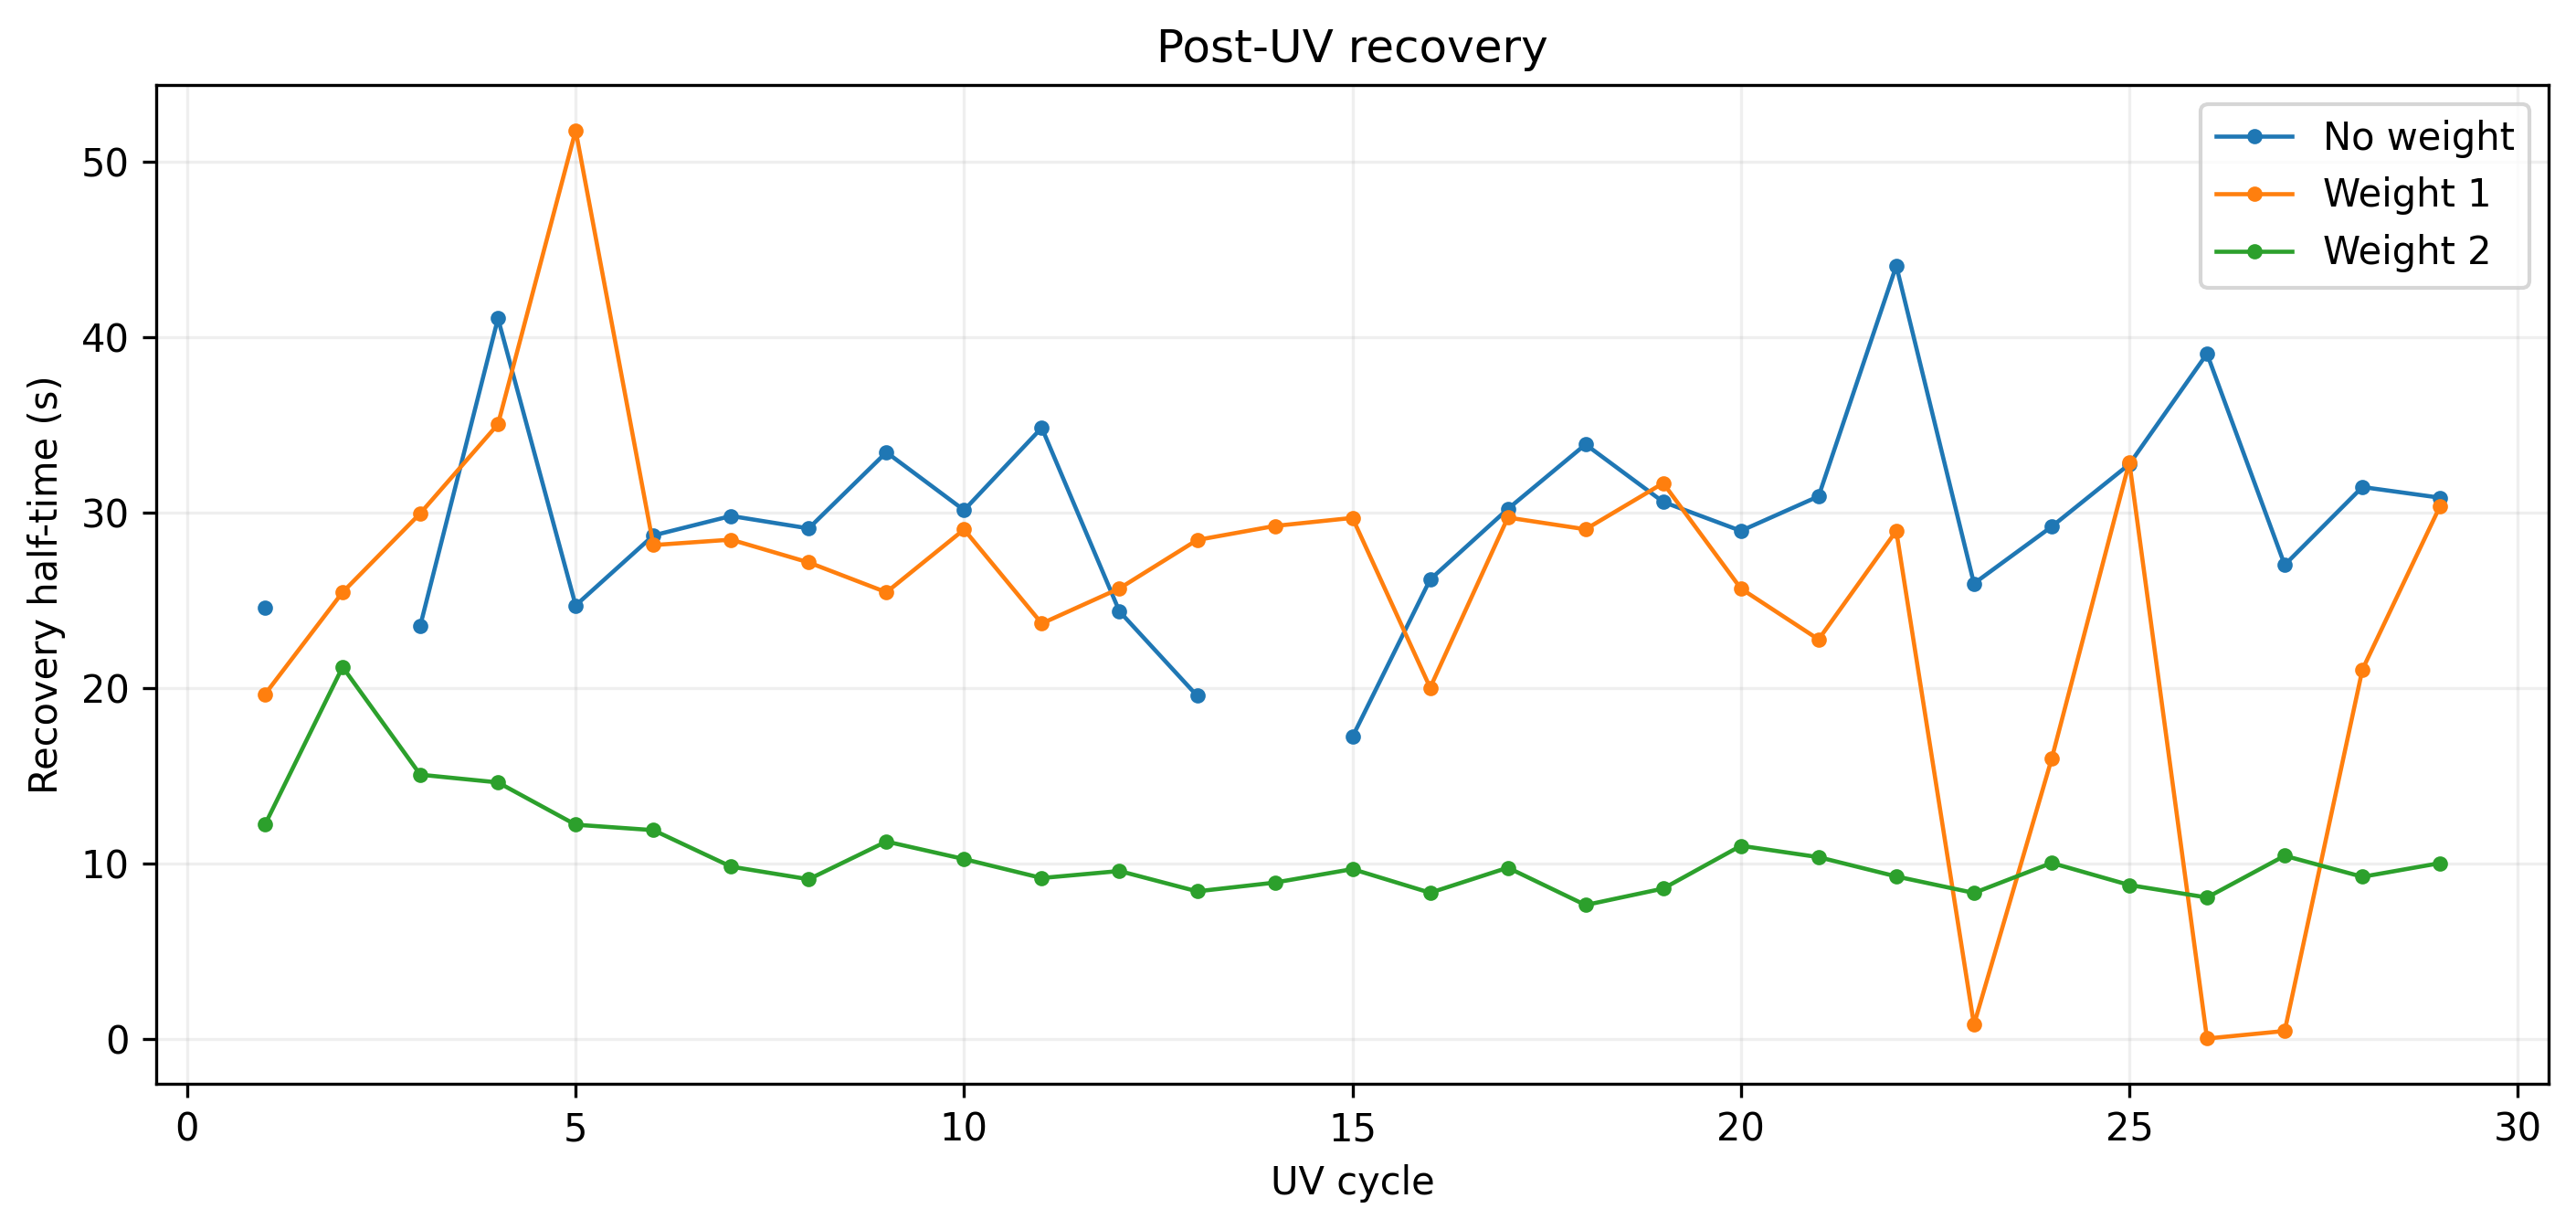
\includegraphics[width=\textwidth]{figures/Figure_3_recovery_half_s.png}
\caption{Post-UV recovery half-time for individual cycles.}
\label{fig:recovery}
\end{figure}

\begin{figure}[H]
\centering
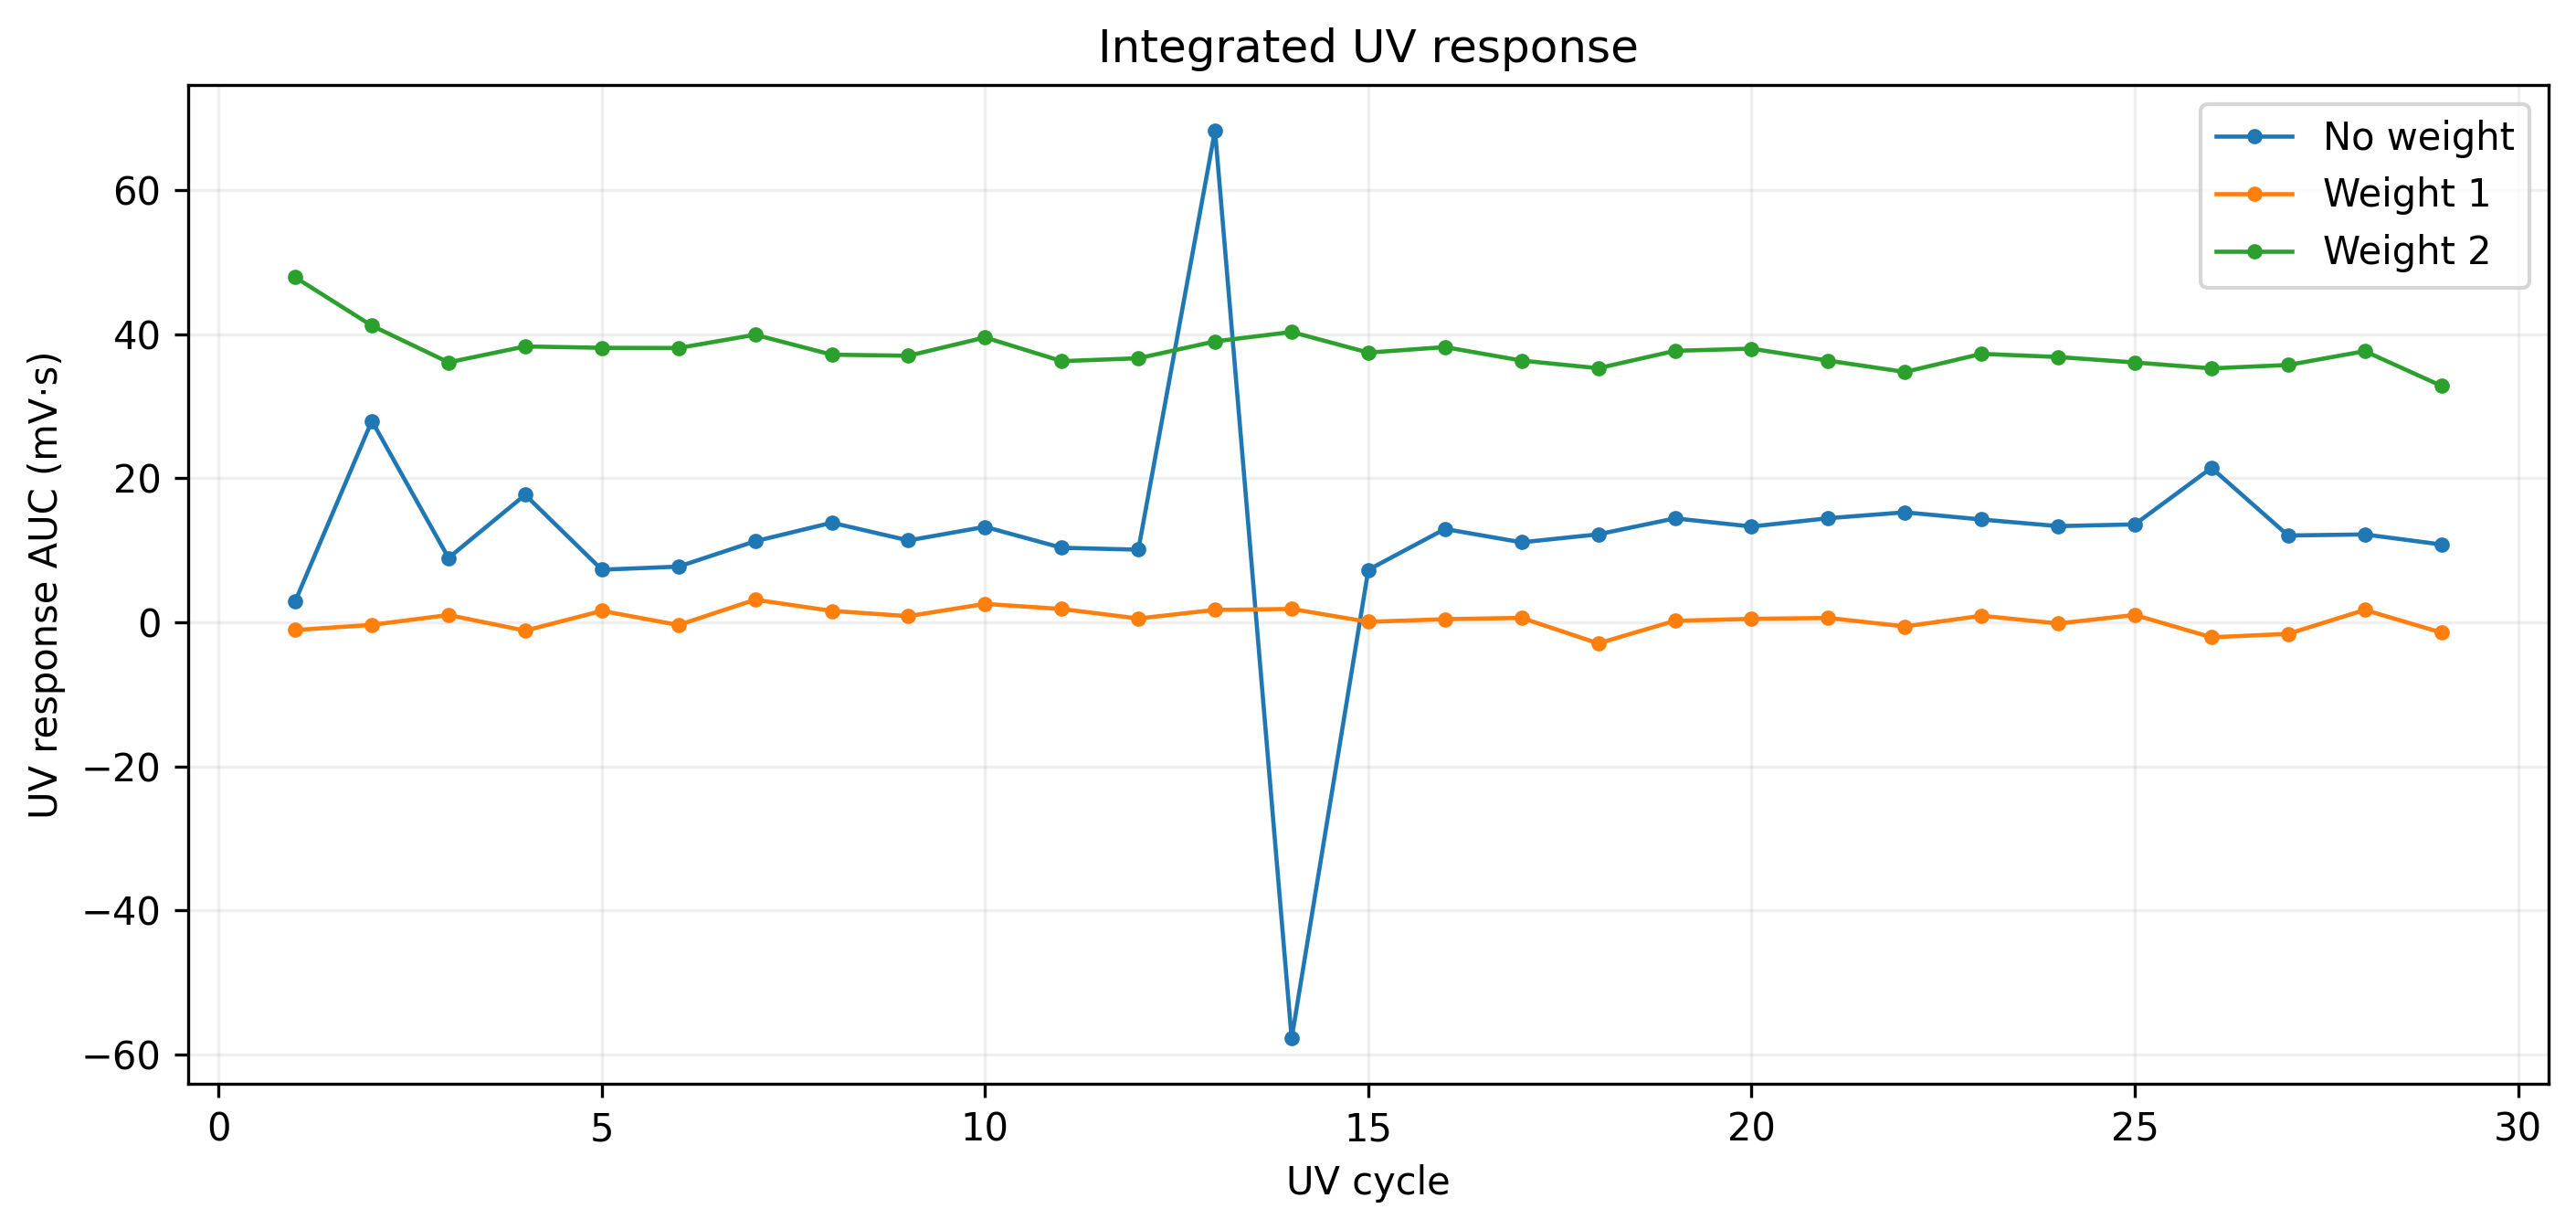
\includegraphics[width=\textwidth]{figures/Figure_3_UV_AUC_mV_s.png}
\caption{Integrated response during the \SI{60}{s} UV exposure.}
\label{fig:auc}
\end{figure}

\section{Cycle-by-cycle response maps}

The heatmaps provide a direct view of the temporal reproducibility of the
response. Each row corresponds to one UV exposure and each column to a
time relative to UV activation.

\begin{figure}[H]
\centering
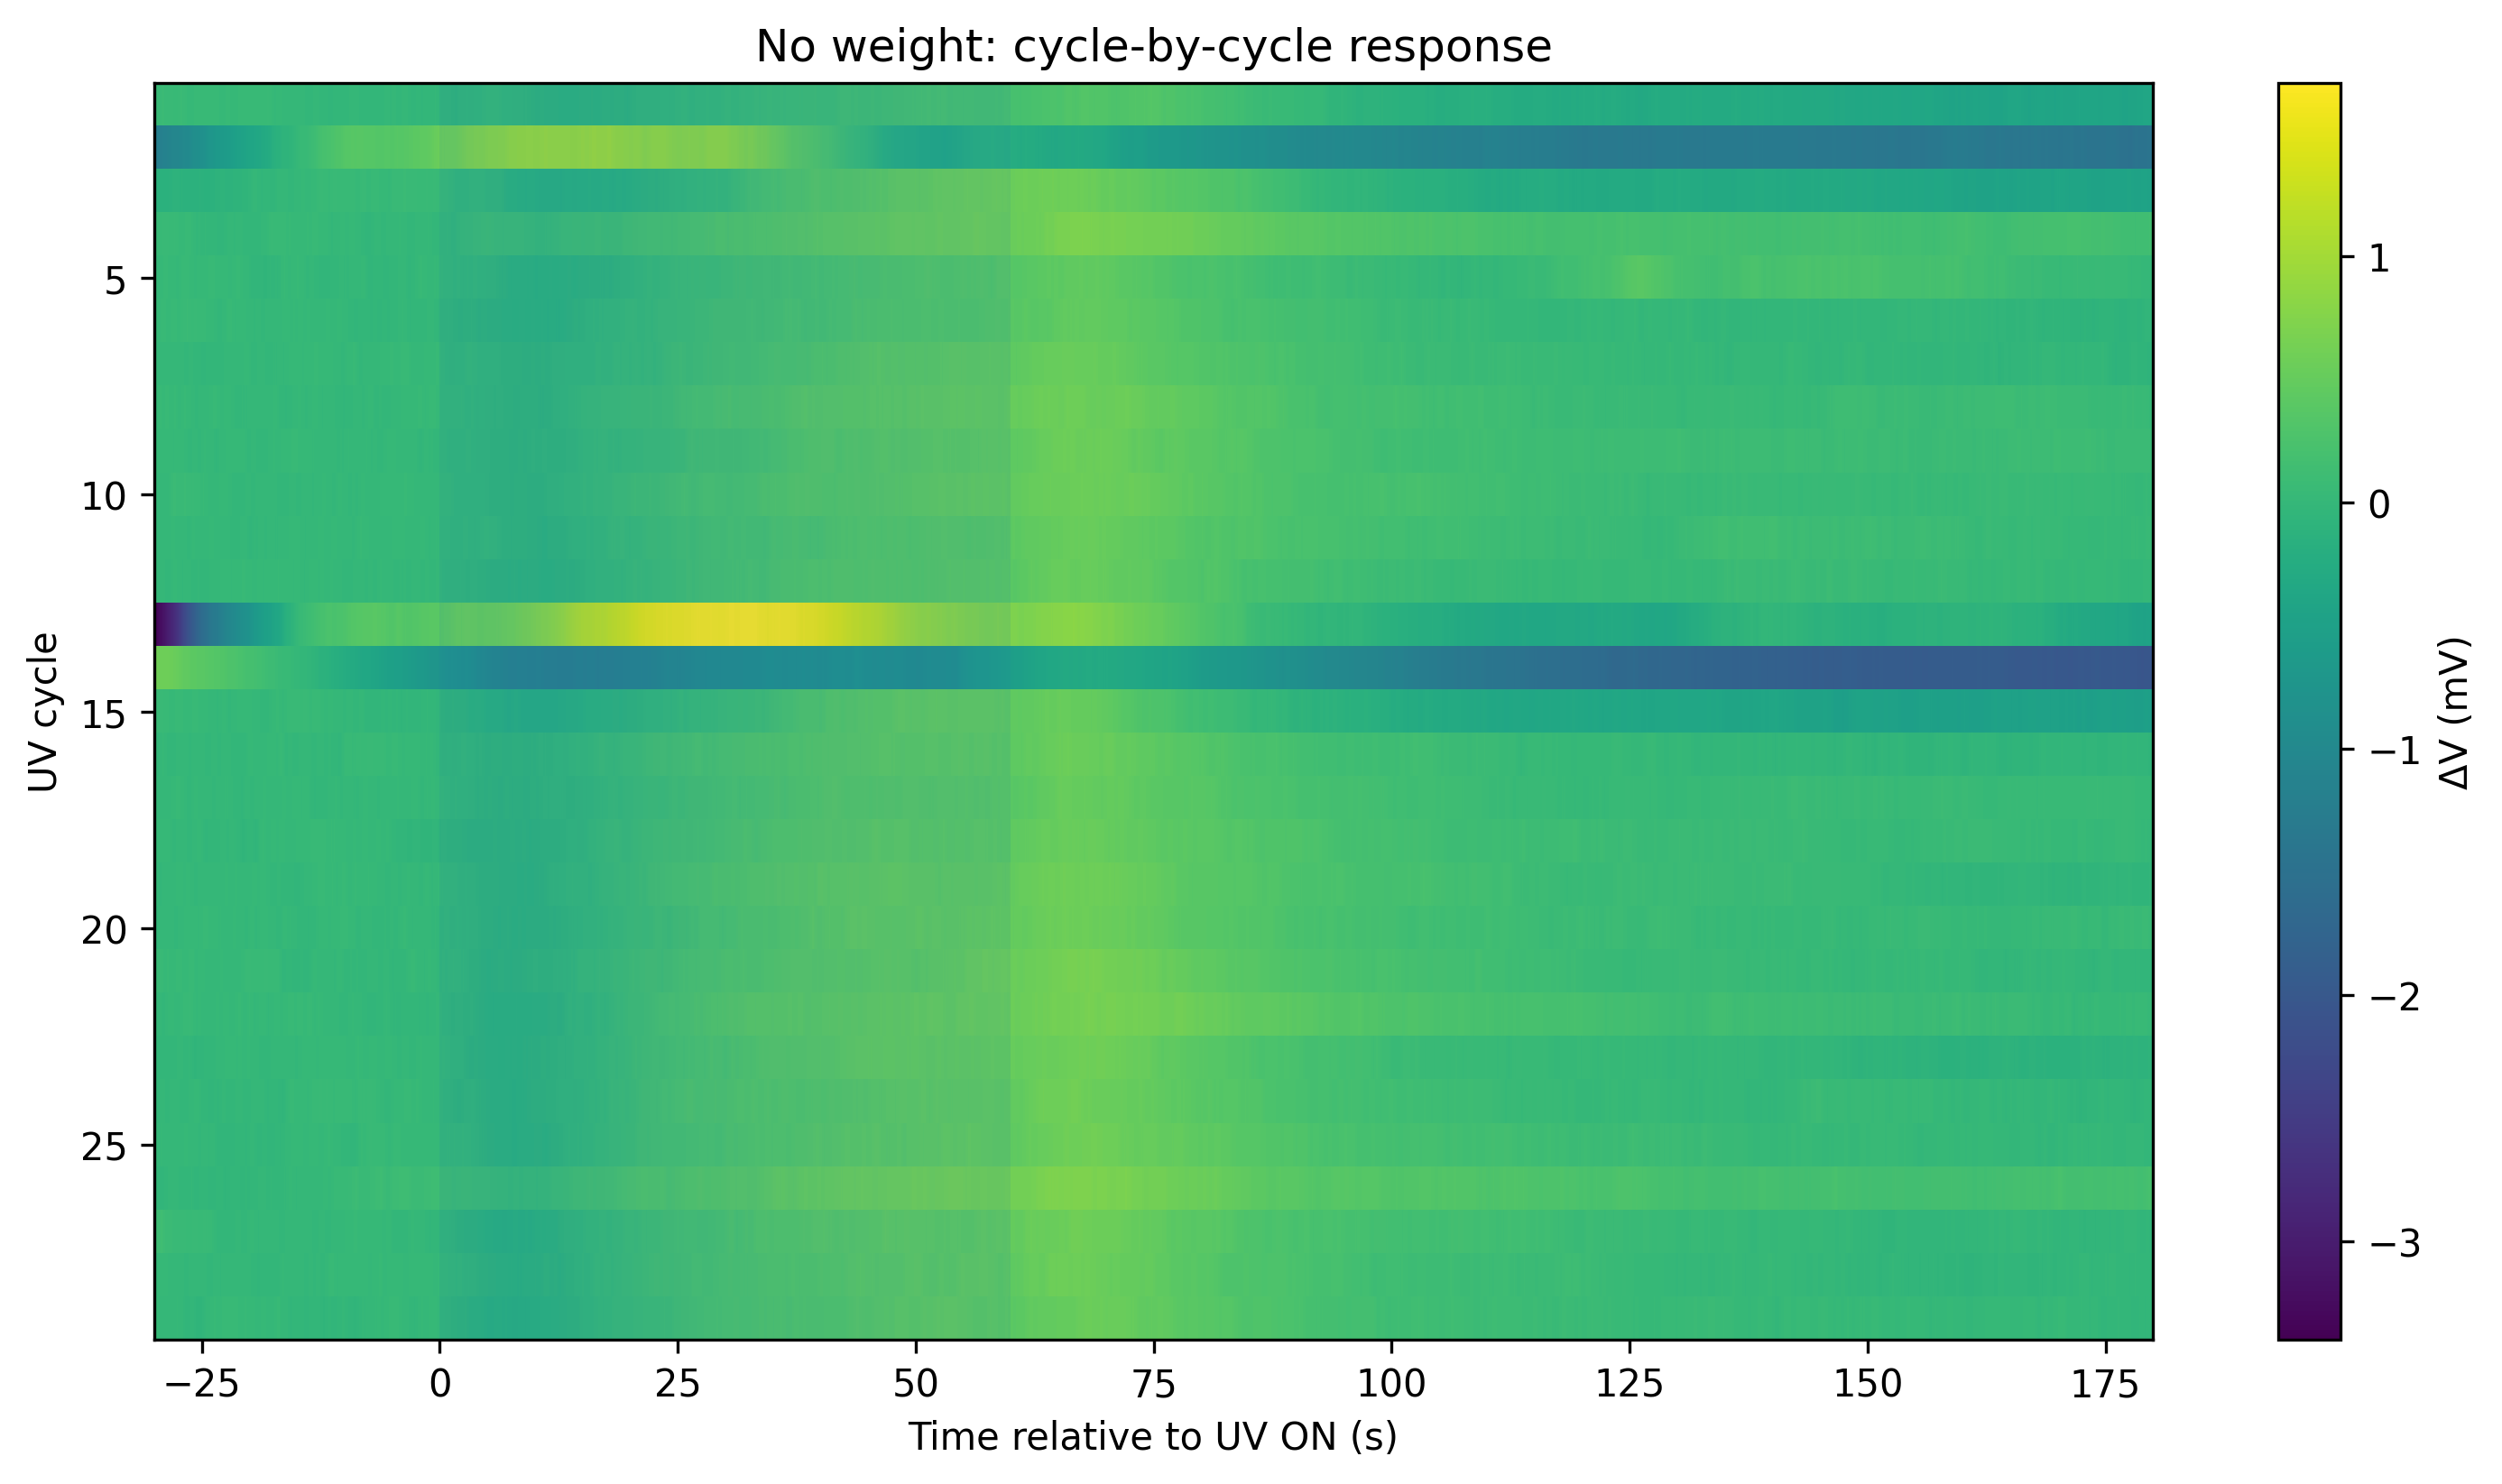
\includegraphics[width=\textwidth]{figures/Figure_4_heatmap_No_weight.png}
\caption{Cycle-by-cycle response matrix for the unloaded recording.}
\label{fig:heat_no}
\end{figure}

\begin{figure}[H]
\centering
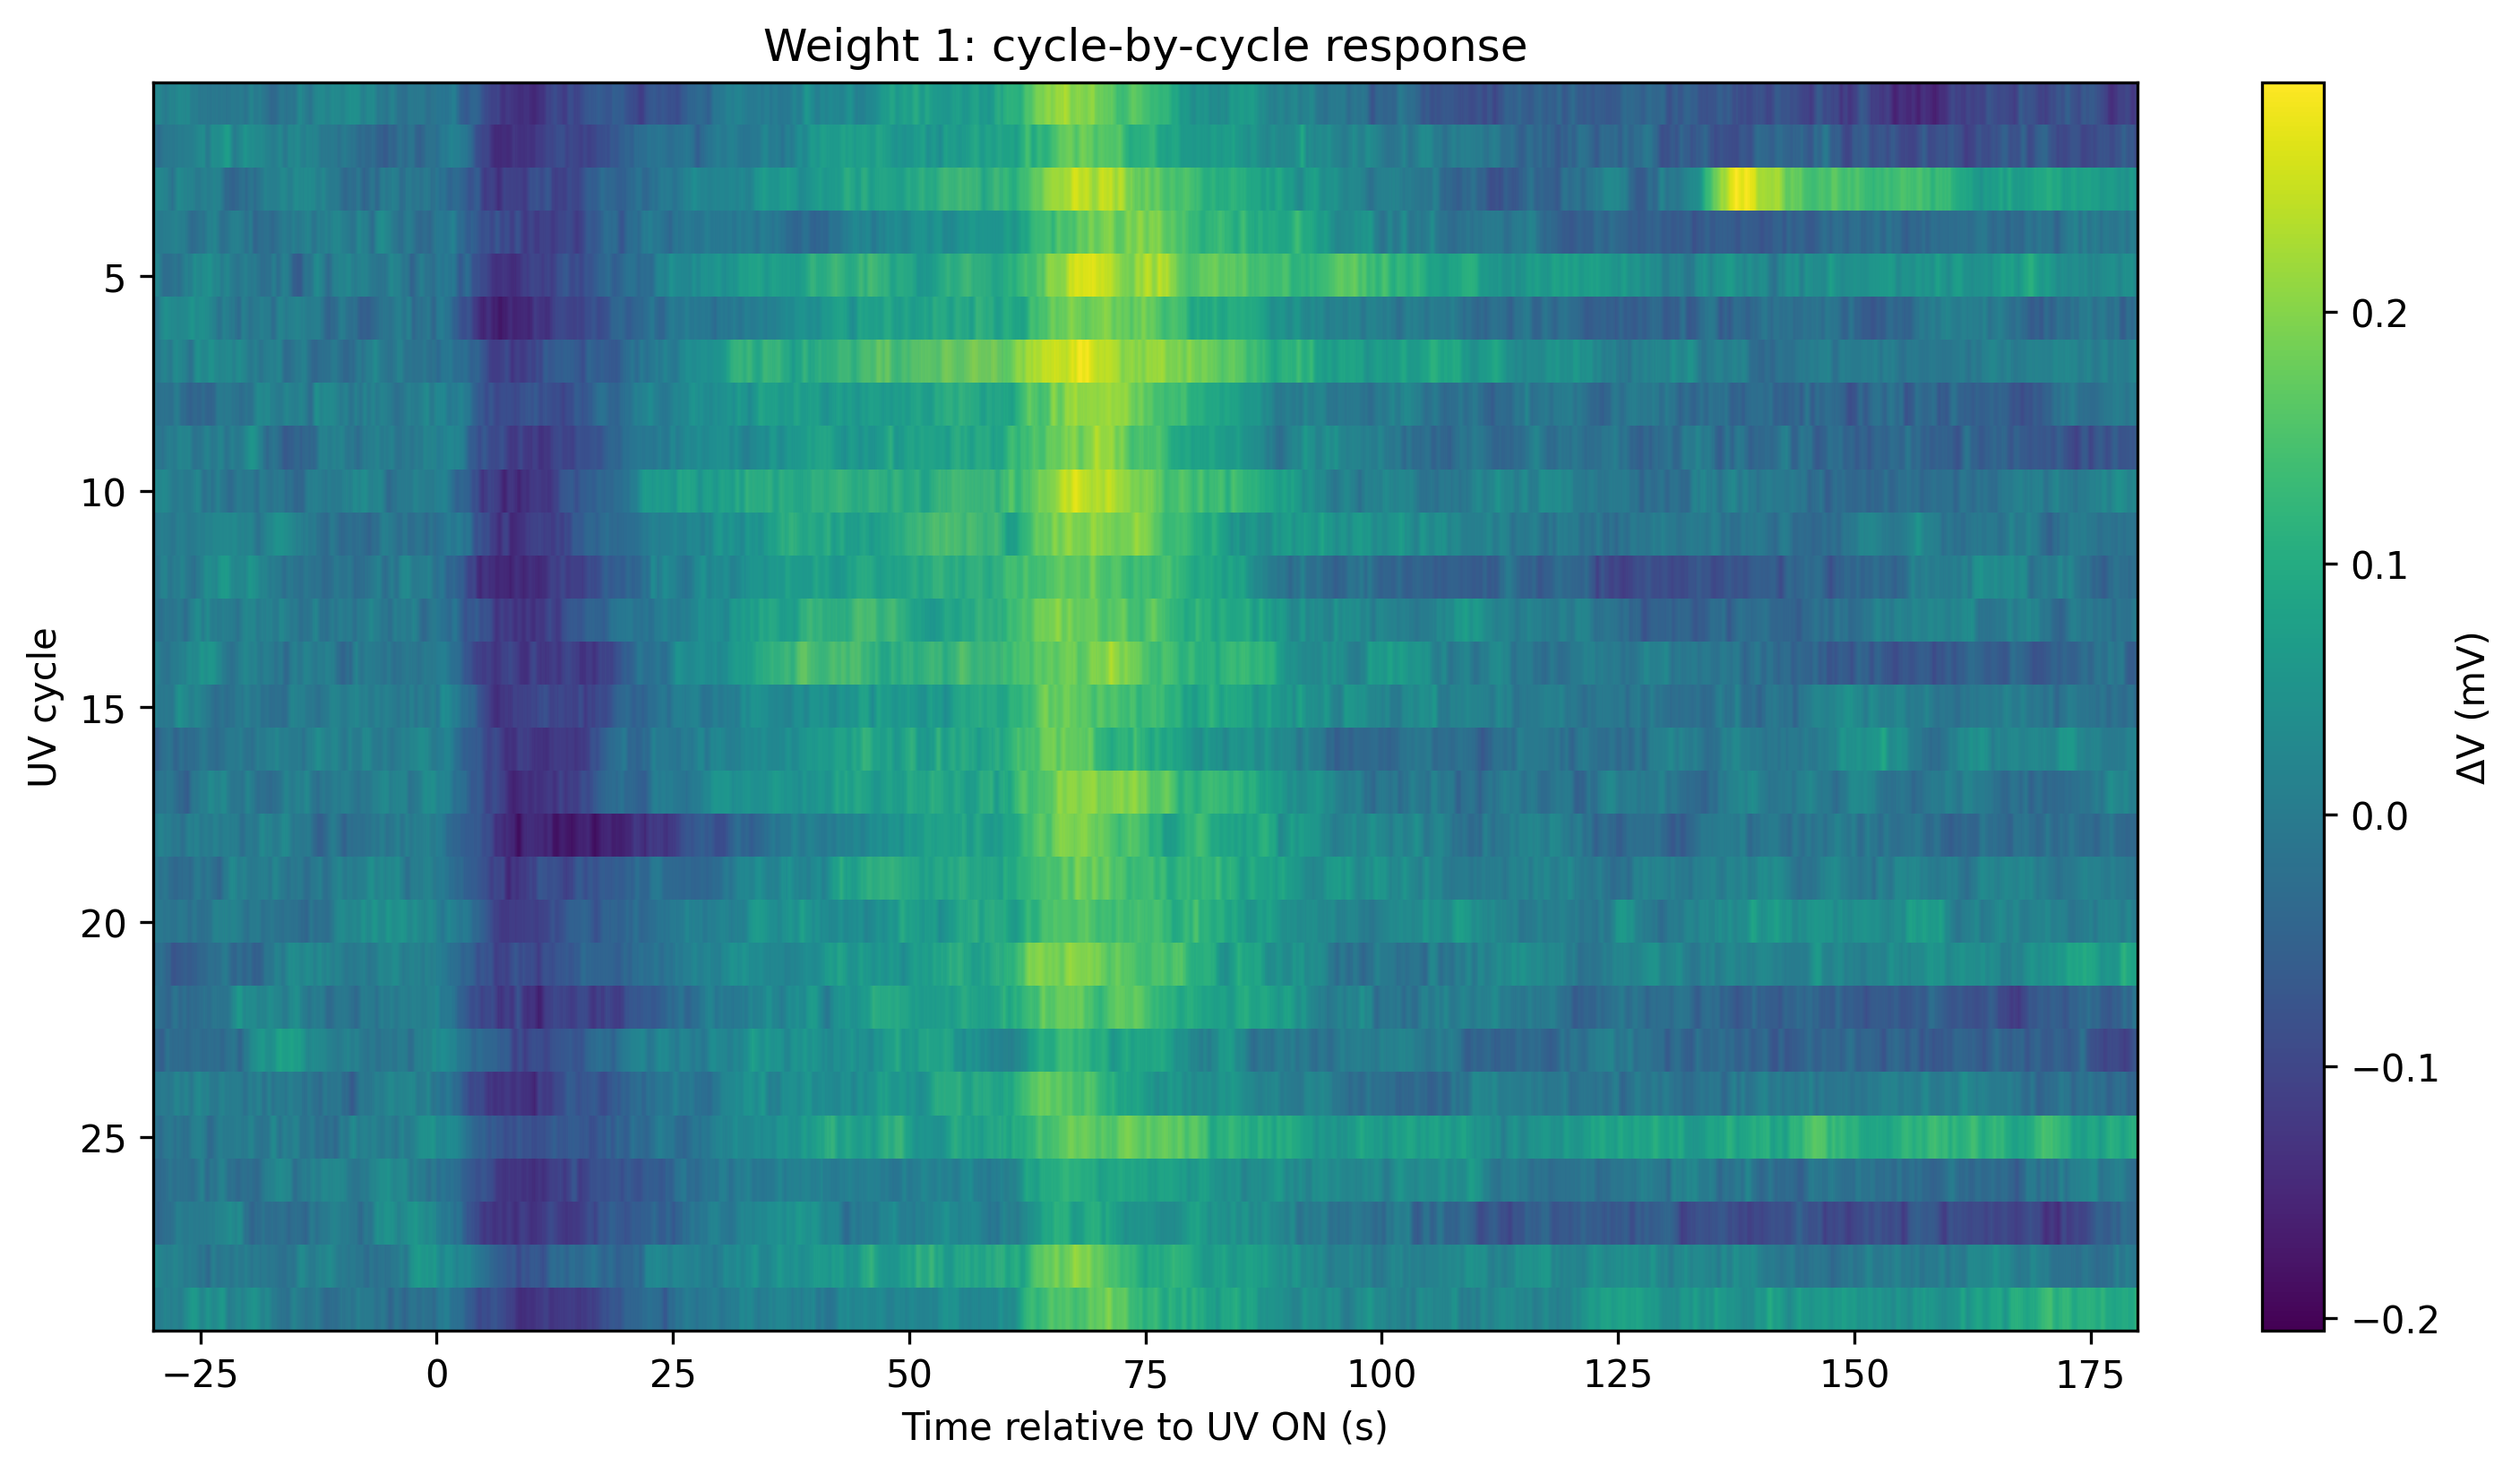
\includegraphics[width=\textwidth]{figures/Figure_4_heatmap_Weight_1.png}
\caption{Cycle-by-cycle response matrix for loaded replicate 1.}
\label{fig:heat_w1}
\end{figure}

\begin{figure}[H]
\centering
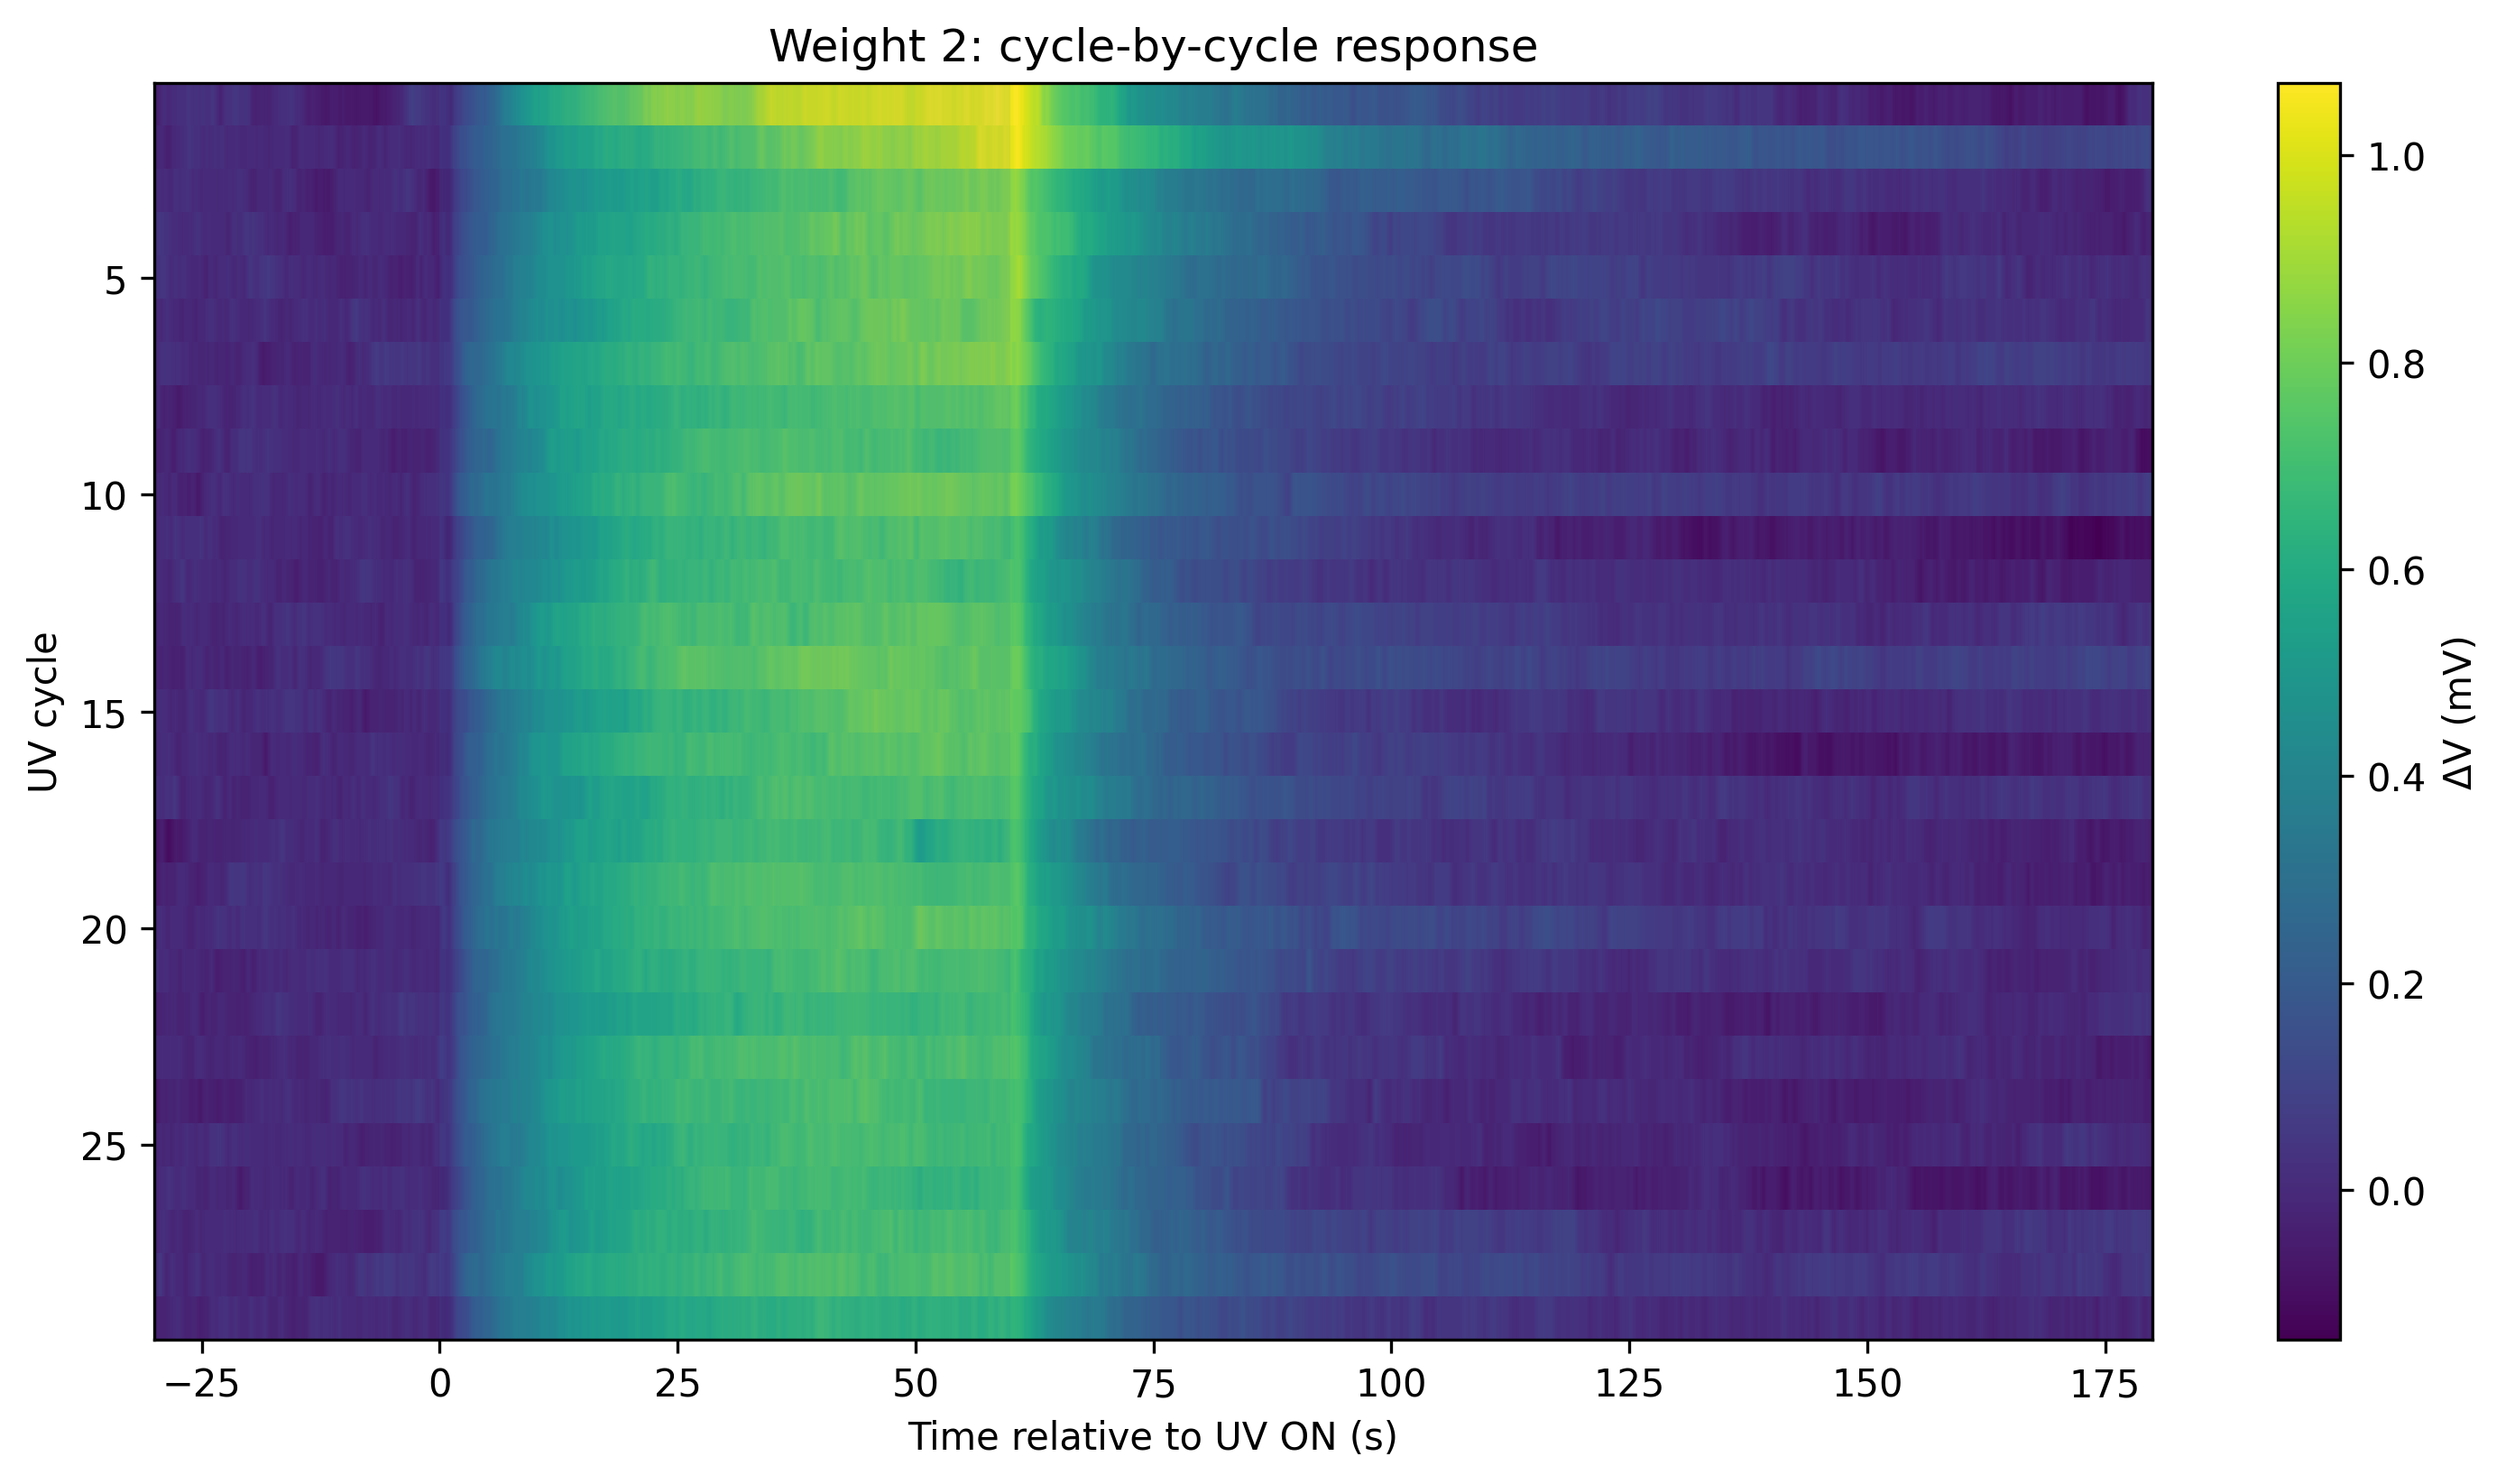
\includegraphics[width=\textwidth]{figures/Figure_4_heatmap_Weight_2.png}
\caption{Cycle-by-cycle response matrix for loaded replicate 2.}
\label{fig:heat_w2}
\end{figure}

The heatmaps show that the second loaded recording is particularly
repeatable in waveform. Its amplitude decreases over the sequence of
repeated exposures, while the temporal structure remains recognizable.
The unloaded recording contains several anomalous cycles, notably around
cycles 2 and 13--14, which should be retained in the raw data but flagged
for quality-control analysis rather than interpreted automatically as large
UV responses.

\section{Kinetic summary}

The numerical summary below is generated directly from the Python analysis
script. It is included through a separate generated LaTeX table so that the
report remains reproducible when the raw data or processing parameters are
changed.

\begin{table}[H]
\centering
\caption{Cycle-level kinetic descriptors. Values are means across the
available complete-recovery cycles; SD denotes the standard deviation across
cycles. These are within-experiment repeated measurements and should not be
interpreted as independent biological replicates.}
\label{tab:kinetics}
\begin{tabular}{lrrrrr}
\hline
Condition & $A_{\max}$ (mV) & $t_{50}$ (s) & $t_{90}$ (s) & $t_{1/2,\mathrm{rec}}$ (s) & UV AUC (mV s)\\
\hline
No weight & 0.471 & 27.2 & 45.1 & 29.9 & 12.55\\
Weight 1 & 0.108 & 33.9 & 44.9 & 29.2 & 0.38\\
Weight 2 & 0.773 & 7.8 & 25.1 & 9.3 & 37.22\\
\hline
\end{tabular}

\end{table}

\section{Comparison with Mishra et al. (Science Robotics, 2024)}

A particularly relevant comparison is provided by Mishra et al.,
\emph{``Sensorimotor control of robots mediated by electrophysiological
measurements of fungal mycelia,''} published in \emph{Science Robotics} in
2024 \cite{Mishra2024}. The paper demonstrates that fungal mycelia can produce
electrophysiological signals in response to environmental stimulation and
uses those signals for biohybrid robotic control. In particular, the authors
use ultraviolet (UV) stimulation to augment robot gaits and report an
experimental electrical response to different UV conditions.

\subsection{1. What they actually demonstrate}

Their overall chain is approximately

\[
\text{UV light}
\;\longrightarrow\;
\text{mycelium electrical response}
\;\longrightarrow\;
\text{signal processing}
\;\longrightarrow\;
\text{artificial control signal}
\;\longrightarrow\;
\text{robot motion}.
\]

The paper demonstrates that UV stimulation produces changes in mycelial
electrophysiological activity and that the resulting signals can be exploited
for robotic control. Their main emphasis is therefore on the use of fungal
electrophysiology as a functional control signal, rather than on a systematic
characterization of how mechanical loading modifies the underlying
stimulus--response relationship. The paper reports UV tests involving
variable UV intensity and exposure time, and quantifies quantities including
changes in electrical potential and peak width. For example, the reported
measurements include electrical-potential changes of several hundred
microvolts and characteristic peak widths on the order of seconds
\cite{Mishra2024}.

\subsection{2. What we are doing is different}

Our experiment is much closer to:

\[
\text{UV stimulation} + \text{mechanical loading}
\;\longrightarrow\;
\text{extracellular electrical response of mycelium}.
\]

and we are asking:

\begin{quote}
\emph{How does mechanical loading modify the amplitude and temporal kinetics
of the electrical response to UV stimulation?}
\end{quote}

That is a substantially different scientific question.

\begin{table}[H]
\centering
\small
\begin{tabular}{p{0.25\textwidth}p{0.32\textwidth}p{0.32\textwidth}}
\toprule
& Mishra et al. & Our experiment \\
\midrule
Biological material & Mycelium & Mycelium \\
Electrical measurement & Extracellular electrophysiology & Extracellular voltage \\
UV stimulation & Yes & Yes \\
Repeated stimulation & Yes & Yes \\
Main objective & Biohybrid robot control & Characterize stimulus--response behaviour \\
UV variable & Intensity / exposure & Repeated standardized 60-s UV pulses \\
Mechanical load & Not the central variable & \textbf{Central experimental variable} \\
Agar control & Reference/control experiments & \textbf{Explicit agar control} \\
Main observables & Spikes, voltage changes, spike timing & \textbf{Amplitude + kinetics + recovery + AUC} \\
Cycle-by-cycle analysis & Not the main emphasis & \textbf{Yes} \\
Loading-dependent response & Not investigated as the main question & \textbf{Yes} \\
\bottomrule
\end{tabular}
\caption{Conceptual comparison between the Science Robotics study and the
present exploratory experiment.}
\label{tab:comparison_mishra}
\end{table}

So I would \textbf{not} frame our work as simply reproducing Mishra et al.

\subsection{3. The most interesting connection: their UV response}

This is where our results become particularly interesting.

Mishra et al. show that UV stimulation produces an enhanced electrical
response in mycelium and that the response can be exploited as a control
signal \cite{Mishra2024}.

Our data independently show a clear UV-locked response. For example, in our
\textbf{Weight 2} experiment:

\begin{itemize}
    \item UV ON $\rightarrow$ rapid positive electrical response;
    \item response reaches roughly \SI{0.77}{mV};
    \item $t_{50}\approx\SI{7.8}{s}$;
    \item $t_{90}\approx\SI{25.1}{s}$;
    \item recovery half-time $\approx\SI{9.3}{s}$.
\end{itemize}

Whereas the \textbf{no-weight} experiment has:

\begin{itemize}
    \item $A_{\max}\approx\SI{0.47}{mV}$;
    \item $t_{50}\approx\SI{27.2}{s}$;
    \item $t_{90}\approx\SI{45.1}{s}$;
    \item recovery half-time $\approx\SI{29.9}{s}$.
\end{itemize}

So the interesting observation is not simply:

\begin{quote}
\emph{``UV causes an electrical signal.''}
\end{quote}

That is already established by Mishra et al.

It is:

\begin{quote}
\textbf{The temporal phenotype of the UV-induced electrical response appears
to depend strongly on mechanical loading.}
\end{quote}

That is much more interesting scientifically.

\subsection{4. There is an important difference in timescale}

This is something to emphasize if we write a paper.

Mishra et al. are particularly interested in action-potential-like spikes and
their use as digital/robotic control signals. Their UV stimulation produces
relatively rapid electrical events, with characteristic peak widths on the
order of seconds \cite{Mishra2024}.

Our analysis is looking at a different component of the response: the slower
transient envelope associated with the 60-s illumination protocol.

Our 60-s illumination produces a \textbf{much slower transient envelope}.
For example, our no-weight response is approximately:

\[
\begin{array}{c}
\text{UV ON}\hspace{4cm}\text{UV OFF}\\[-1mm]
\downarrow\hspace{4.2cm}\downarrow
\end{array}
\]

\[
V(t)\;\sim\;
\text{slow rise during illumination}
\;\longrightarrow\;
\text{recovery after UV OFF}.
\]

Whereas their application is much more concerned with detecting the discrete
electrical events and converting them into control commands.

This suggests that we may be measuring a \textbf{different level of the
biological response} rather than competing with their spike-based
measurement.

\subsection{5. The really interesting result may be Weight 2}

Looking at our results in light of their paper changes how we would interpret
our experiment.

Initially we were asking:

\begin{quote}
\emph{Does weight increase or decrease the voltage?}
\end{quote}

I now think that is \textbf{too simplistic}.

Our data suggest that loading may alter at least three independent
properties:

\paragraph{Amplitude}
\[
A_{\max}.
\]
Weight 2:
\[
0.773\ \mathrm{mV}
\]
No weight:
\[
0.471\ \mathrm{mV}.
\]

\paragraph{Response speed}
\[
t_{50}.
\]
Weight 2:
\[
7.8\ \mathrm{s}
\]
No weight:
\[
27.2\ \mathrm{s}.
\]

\paragraph{Recovery speed}
\[
t_{1/2,\mathrm{rec}}.
\]
Weight 2:
\[
9.3\ \mathrm{s}
\]
No weight:
\[
29.9\ \mathrm{s}.
\]

So the striking thing is actually:

\begin{quote}
\textbf{Weight 2 does not merely produce a larger response; it produces a
qualitatively faster response.}
\end{quote}

That is potentially much more interesting.

\subsection{6. And this gives us a better scientific hypothesis}

Instead of:

\begin{quote}
\emph{Mechanical loading affects the electrical response of mycelium to UV.}
\end{quote}

I would formulate the hypothesis as:

\[
\boxed{
\text{Mechanical loading modulates the amplitude and temporal kinetics of
UV-induced mycelial electrophysiological responses.}
}
\]

Then we have measurable quantities:

\[
\{A_{\max},t_{50},t_{90},t_{\mathrm{rec}},\mathrm{AUC}\}.
\]

This is much stronger experimentally.

\subsection{7. Our agar control becomes especially important}

The Science Robotics paper establishes that mycelium responds to UV, but our
experiment has another useful element: \textbf{agar without mycelium}.

Our agar response does not reproduce the strong sustained positive response
seen particularly in Weight 2.

For example, approximately:

\begin{table}[H]
\centering
\begin{tabular}{lrr}
\toprule
 & Agar & Weight 2 \\
\midrule
0--20 s & $-0.05$ mV & $+0.57$ mV \\
40--60 s & $-0.09$ mV & $+1.02$ mV \\
60--80 s & $-0.13$ mV & $+0.64$ mV \\
\bottomrule
\end{tabular}
\caption{Descriptive comparison of representative baseline-subtracted UV-cycle
windows for the agar control and Weight 2 experiment.}
\label{tab:agar_weight2}
\end{table}

So this gives us an important control against simply saying:

\begin{quote}
\emph{UV + conductive/moist biological substrate = voltage artifact.}
\end{quote}

It supports the interpretation that the large positive response is associated
with the \textbf{presence of living mycelium}, although it does not by itself
establish the precise biological mechanism.

\subsection{8. There is also a methodological lesson from their paper}

Their work puts considerable emphasis on obtaining stable electrophysiological
measurements and shielding the measurement from vibration and electromagnetic
interference \cite{Mishra2024}.

That is relevant to us.

Our next experiment should therefore make the distinction between

\[
V_{\mathrm{measured}}
=
V_{\mathrm{biological}}
+
V_{\mathrm{UV/artifact}}
+
V_{\mathrm{mechanical}}
+
V_{\mathrm{electrical\ noise}}
\]

as cleanly as possible.

\subsection{9. Where I think our work could go beyond the Science Robotics
paper}

This is the part I find most promising.

We could construct a \textbf{stimulus--mechanics--electrical response map}:

\[
\boxed{
(L,I_{\mathrm{UV}},T_{\mathrm{UV}})
\longrightarrow
V(t)
}
\]

where

\begin{itemize}
    \item $L$ = mechanical load;
    \item $I_{\mathrm{UV}}$ = UV intensity;
    \item $T_{\mathrm{UV}}$ = exposure duration.
\end{itemize}

and then reduce $V(t)$ to:

\[
A,\quad t_{50},\quad t_{90},\quad
t_{\mathrm{recovery}},\quad \mathrm{AUC}.
\]

That turns the mycelium into something closer to an \textbf{engineered living
transducer}.

Conceptually:

\[
\boxed{
\text{Mechanical state}
\rightarrow
\text{modulation of biological response}
\rightarrow
\text{electrical signal}
}
\]

while Mishra et al. essentially use:

\[
\boxed{
\text{environmental stimulus}
\rightarrow
\text{mycelial electrical signal}
\rightarrow
\text{robotic actuation}.
}
\]

Those are complementary rather than redundant.

\subsection{10. One major caveat}

We should \textbf{not yet claim that loading causes the differences}.

We currently have:

\begin{itemize}
    \item one no-weight experiment;
    \item one Weight 1 experiment;
    \item one Weight 2 experiment;
    \item repeated UV cycles within each experiment.
\end{itemize}

The 30 cycles are \textbf{not 30 independent biological replicates}.

And, importantly, Weight 1 and Weight 2 behave very differently.

That makes the next experiment particularly important.

I would do something like:

\[
0,\;L_1,\;L_2,\;L_3
\]

with \textbf{at least 3 independent mycelium samples per loading condition},
and perhaps 5--10 UV cycles per sample.

Then we can ask whether

\[
A_{\max}=f(L)
\]

and

\[
t_{50}=g(L)
\]

actually emerge as reproducible relationships.

\subsection{Overall assessment}

The comparison strengthens the rationale for what we are doing.

Mishra et al. have already established the important premise:

\begin{quote}
\emph{mycelium can convert UV stimulation into measurable electrical activity
and that activity can be functionally exploited.}
\end{quote}

Our experiment asks a different and natural next question:

\begin{quote}
\emph{Can the electrical transduction of an environmental stimulus be
modulated by the mechanical state of the living fungal material?}
\end{quote}

Our preliminary data suggest that the answer may be \textbf{yes}, particularly
because the loading condition appears to affect not only amplitude but also
\textbf{response and recovery kinetics}.

We would therefore \textbf{not change our analysis pipeline}. Instead, the
Science Robotics paper can be used to strengthen the scientific framing and
make \textbf{amplitude + kinetics + mechanical loading} the central story.

\section{Combined time-domain and frequency-domain characterization}

The time-domain analysis describes amplitude and kinetics of the UV-induced response. We next treat the experiment as a periodic input--output problem because the UV command is deterministic: \SI{60}{s} ON followed by \SI{180}{s} OFF, repeated every \SI{240}{s}. The fundamental stimulus frequency is
\[
f_0=\frac{1}{240}=\SI{0.004167}{Hz},
\]
with harmonics at integer multiples of $f_0$.

For each complete UV cycle, the filtered voltage was represented by its complex Fourier coefficient $Y_k$ and the known UV command by $U_k$. We formed the descriptive harmonic input--output estimate
\[
H_k=\frac{Y_k}{U_k}.
\]
The magnitude $|H_k|$ describes voltage response per unit UV input at harmonic $k$, while $\arg(H_k)$ describes the phase relationship. This is a descriptive harmonic response, not yet a conventional linear time-invariant transfer function: the biological system may be nonlinear, time-varying, and adaptive.

\begin{figure}[H]\centering
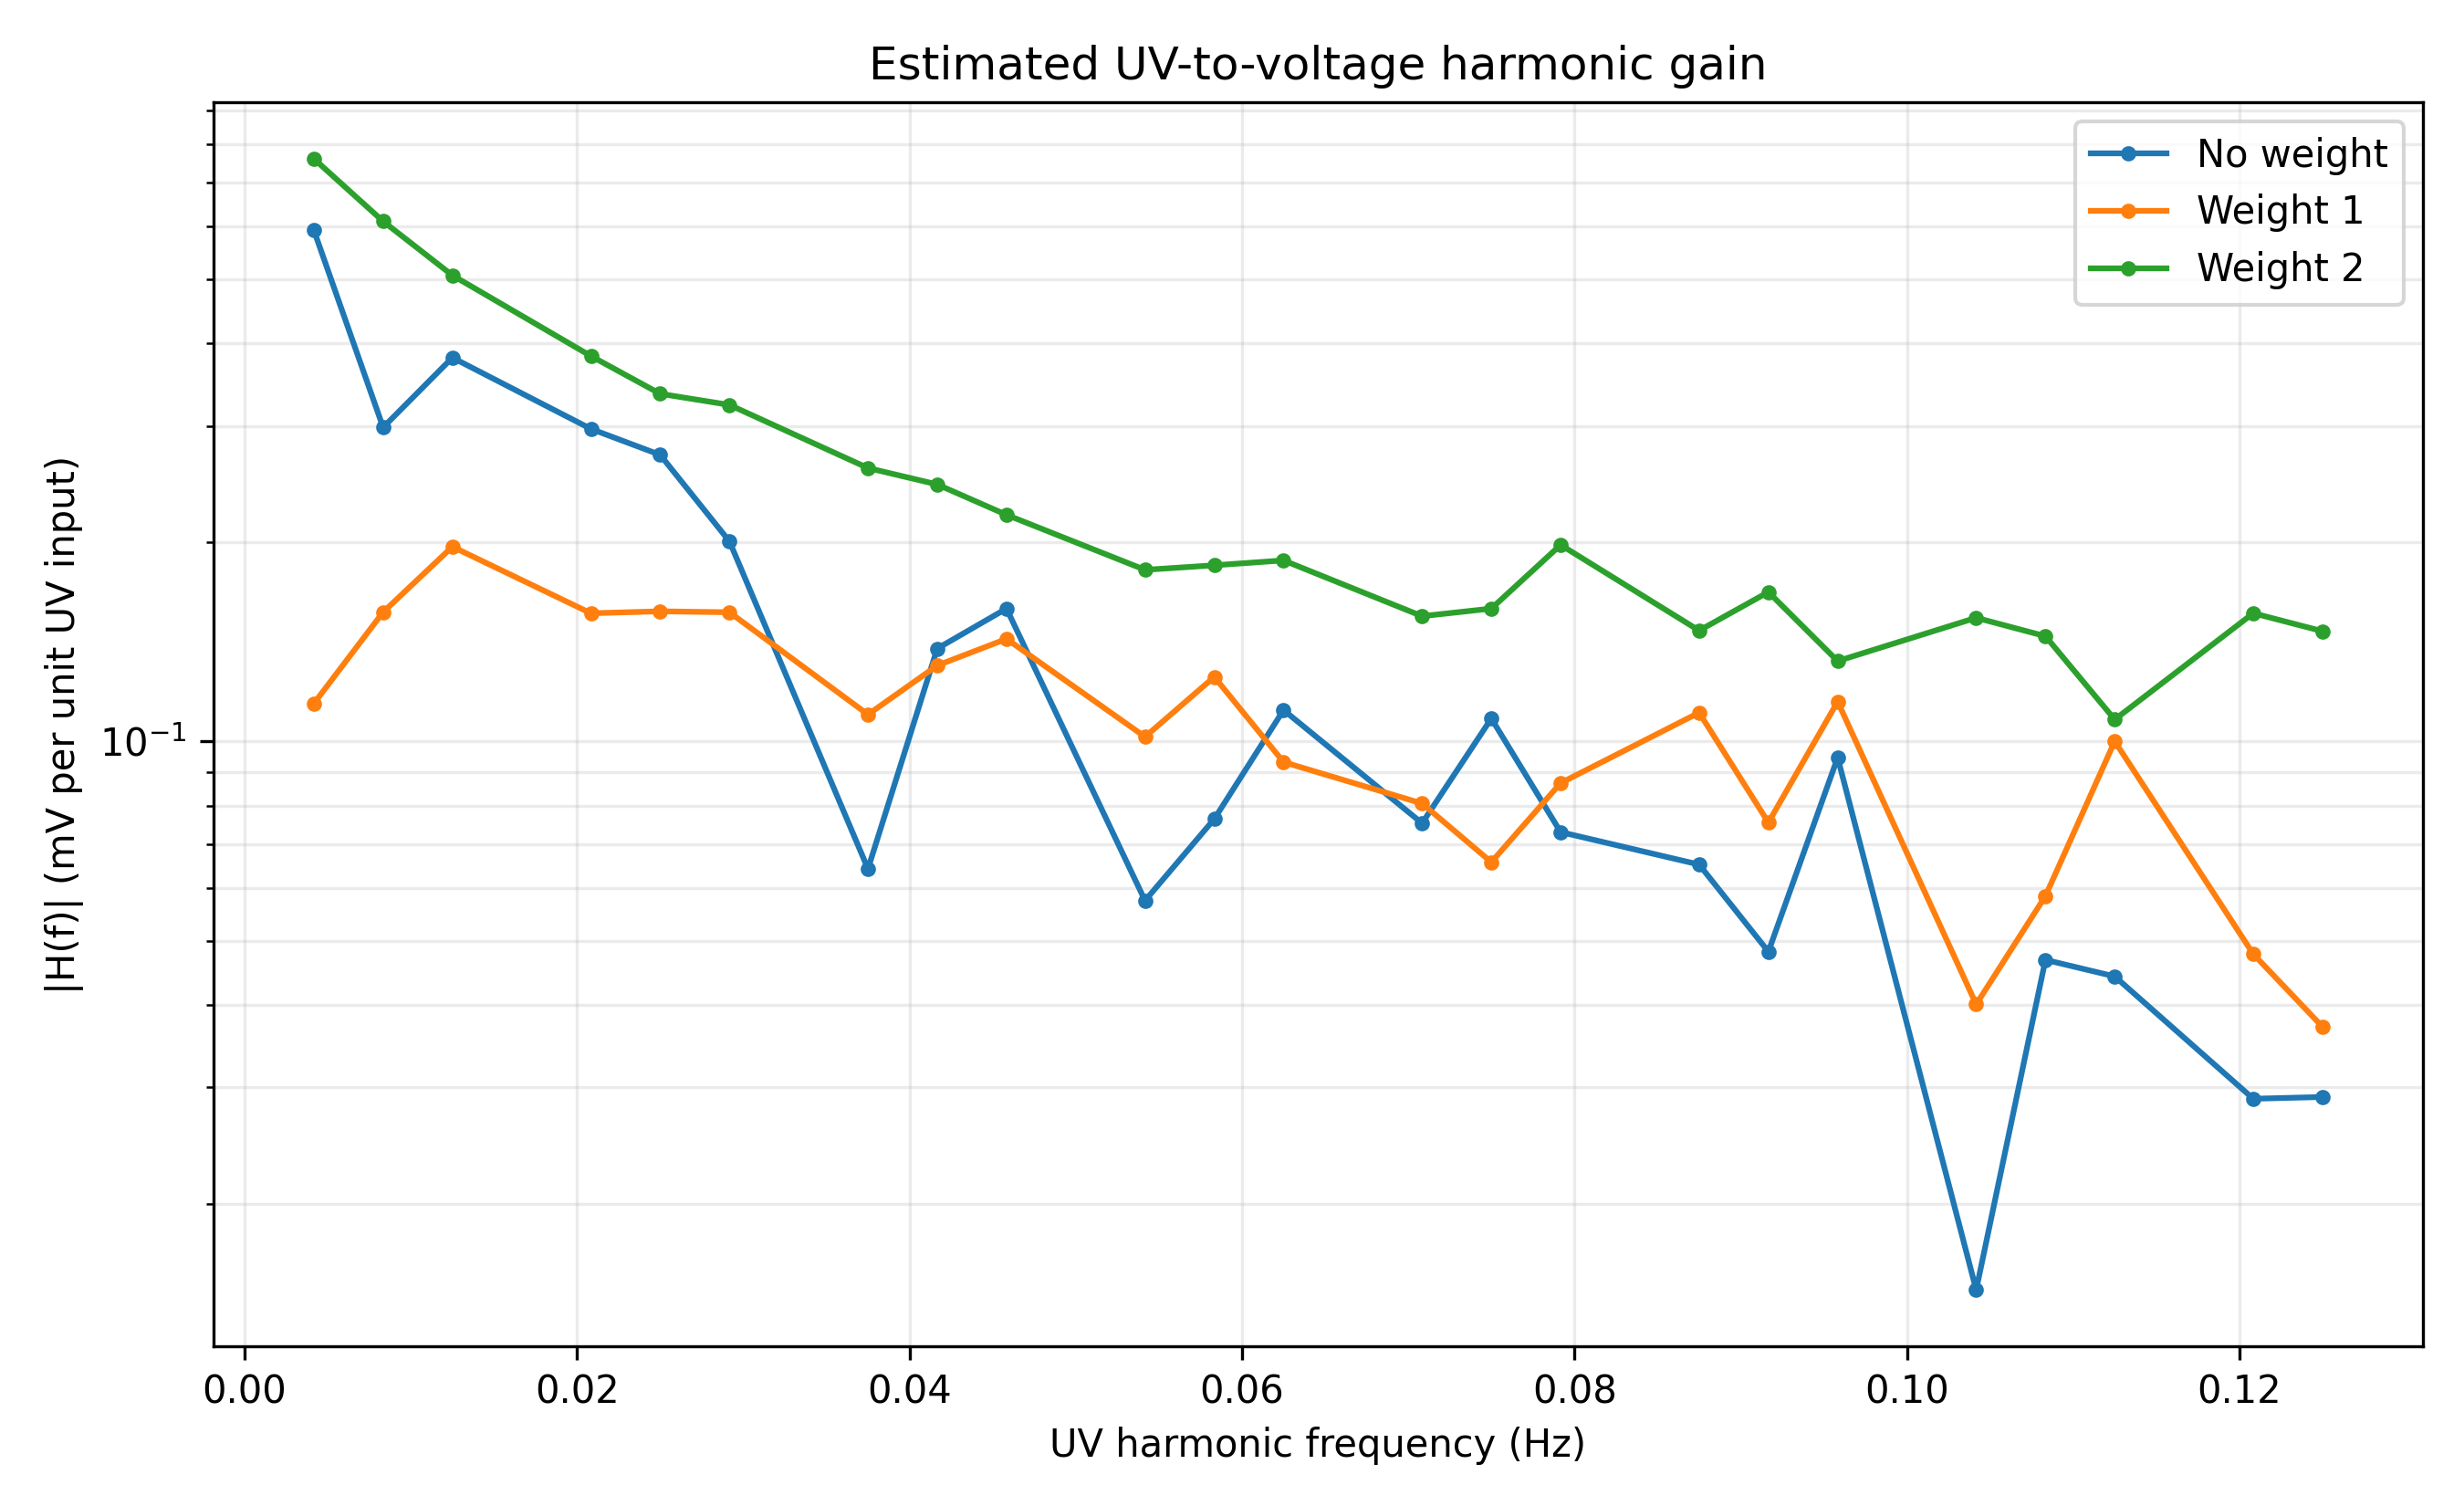
\includegraphics[width=0.92\textwidth]{figures/Figure_9_harmonic_gain.png}
\caption{Estimated UV-to-voltage harmonic gain. The Weight 2 recording exhibits substantially larger gain over the first several harmonics.}\label{fig:harmonic_gain}
\end{figure}

\begin{figure}[H]\centering
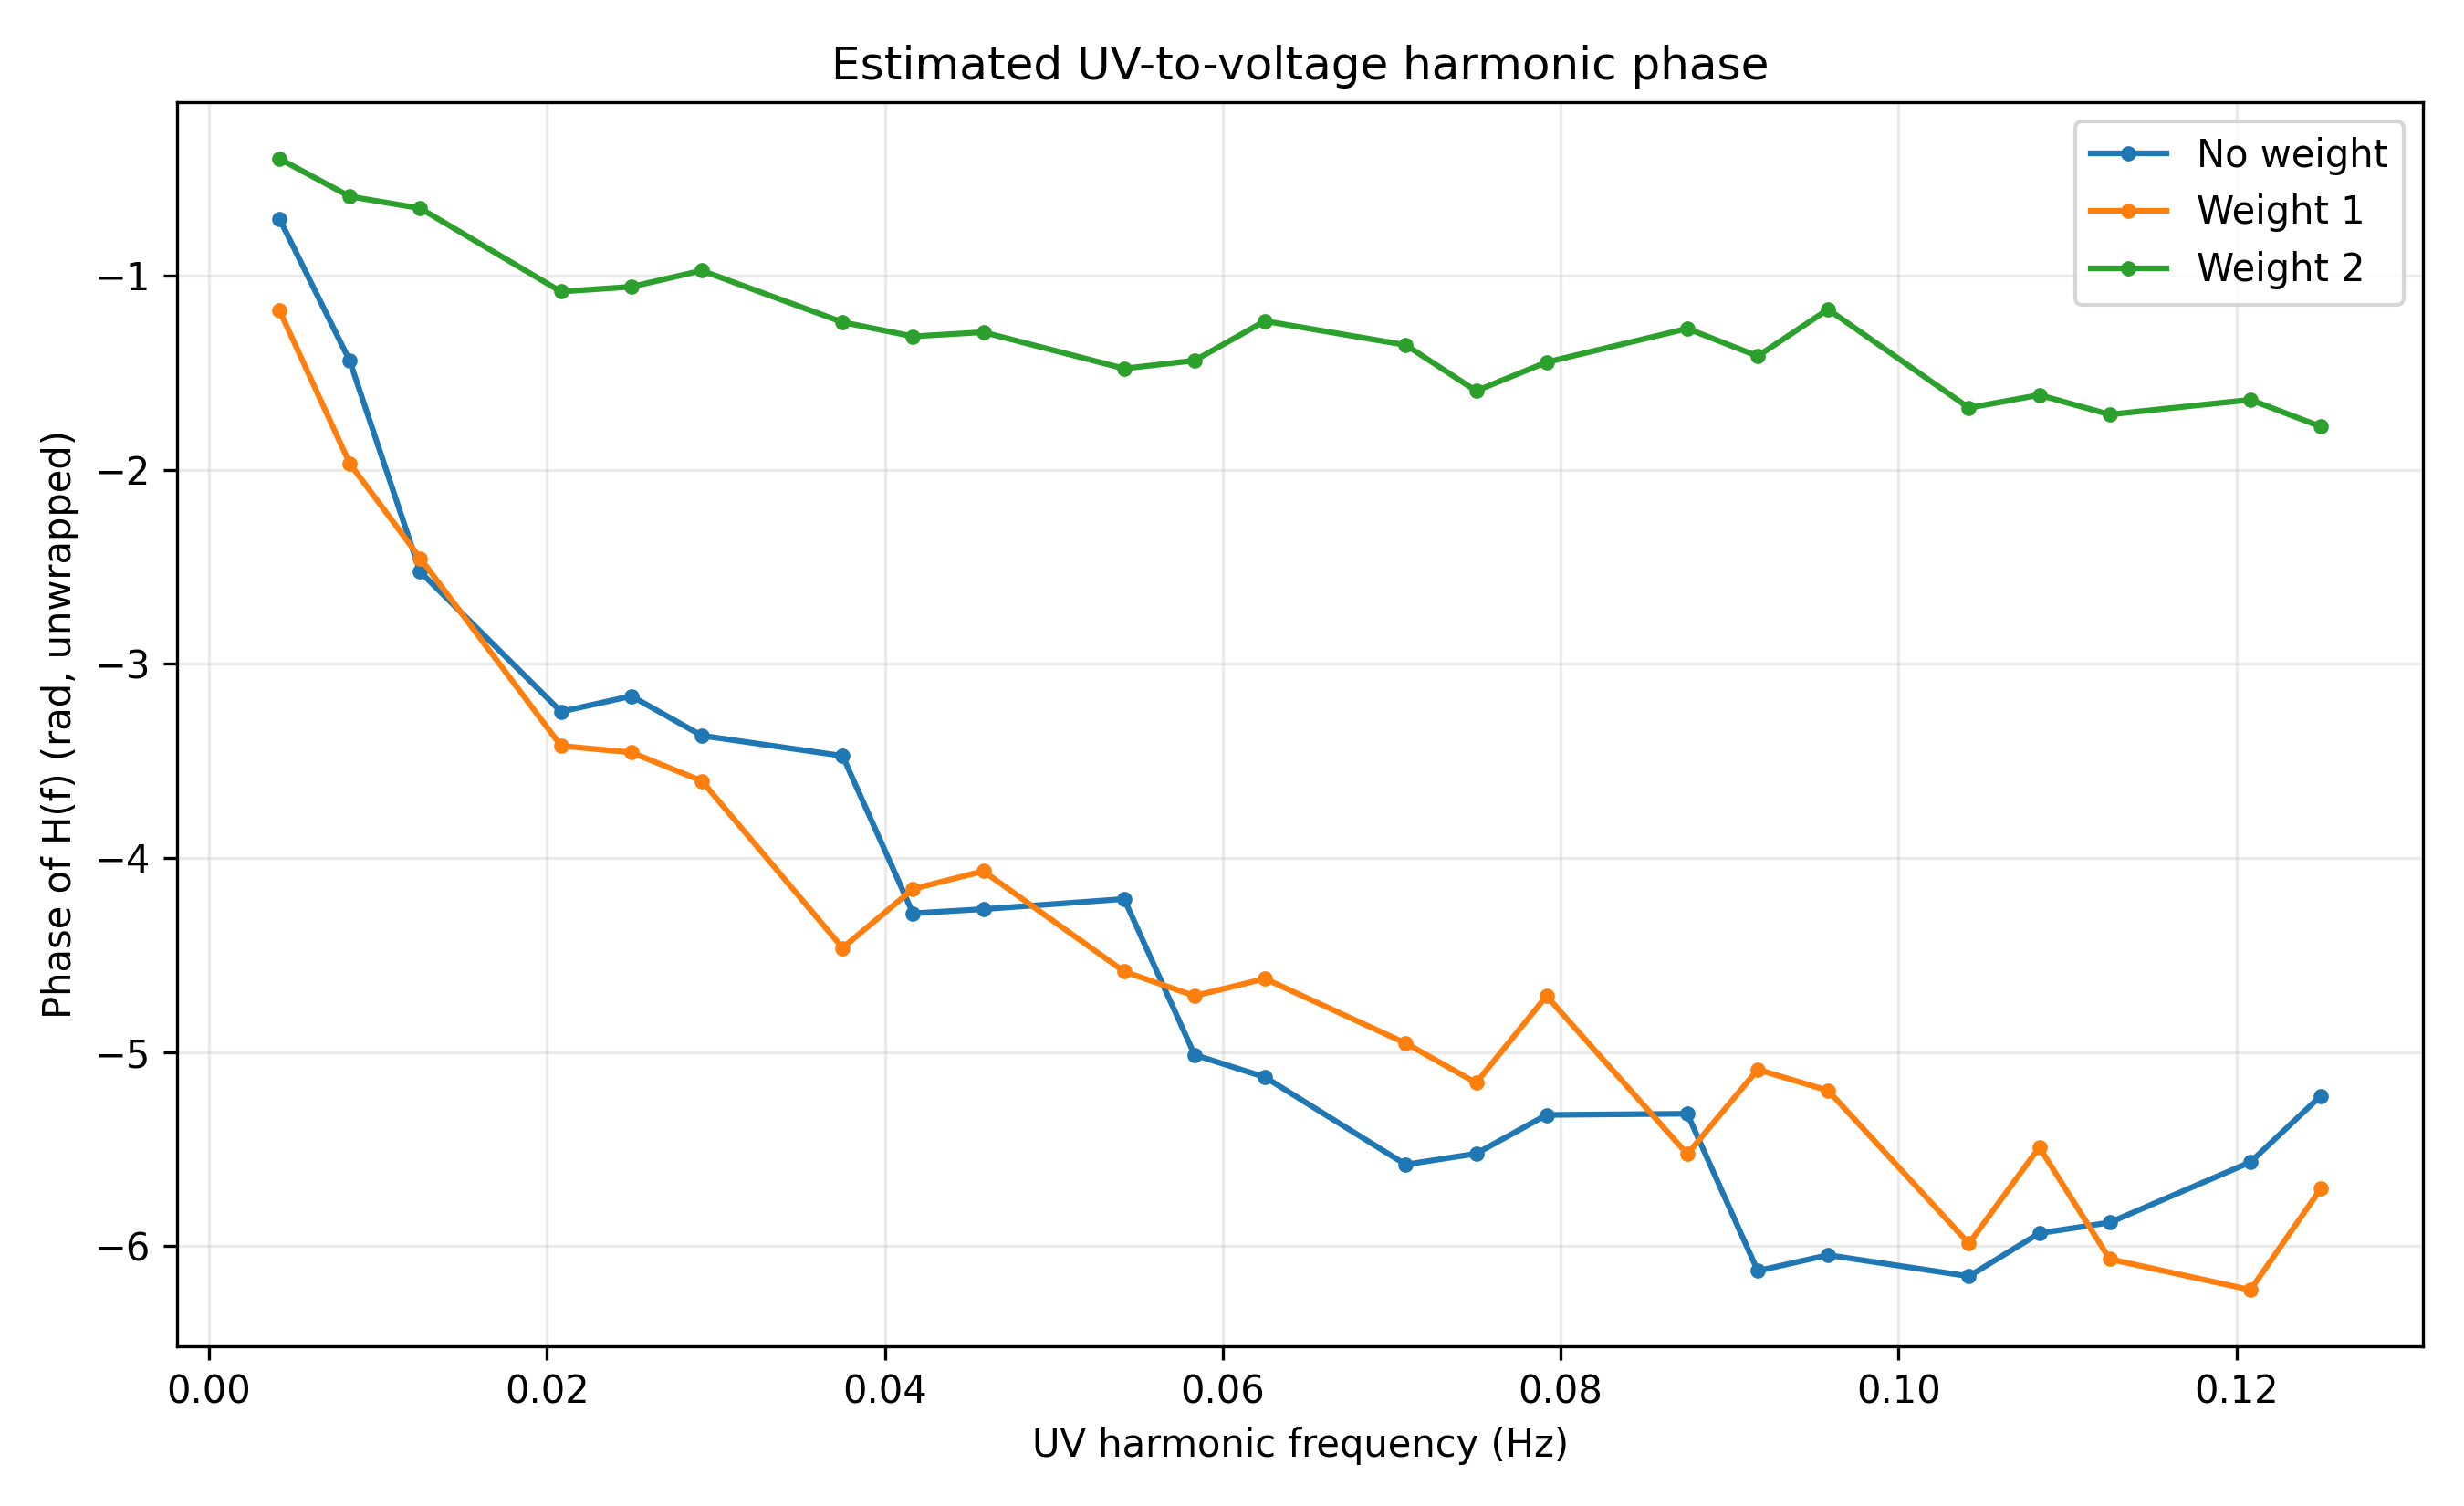
\includegraphics[width=0.92\textwidth]{figures/Figure_10_harmonic_phase.png}
\caption{Estimated phase of the UV-to-voltage harmonic response.}\label{fig:harmonic_phase}
\end{figure}

\subsection{Harmonic gain and coherence}

The first-harmonic results provide a compact comparison:
\begin{table}[H]\centering
\begin{tabular}{lrrr}\toprule
Condition & $|H_1|$ (mV) & Phase (rad) & Coherence\\\midrule
No weight & 0.593 & -0.706 & 0.660\\
Weight 1 & 0.114 & -1.179 & 0.782\\
Weight 2 & \textbf{0.760} & \textbf{-0.398} & \textbf{0.977}\\\bottomrule
\end{tabular}
\caption{Descriptive first-harmonic UV-to-voltage response. Coherence is magnitude-squared coherence at the UV fundamental.}\label{tab:first_harmonic}
\end{table}

The Weight 2 experiment is notable because the observations converge across different descriptions of the same response. In the time domain it has the largest response amplitude, shortest $t_{50}$, shortest recovery half-time, and largest UV AUC. In the frequency domain it also has the largest first-harmonic gain and the highest coherence with the known UV input.

At the first three harmonics, Weight 2 has coherence values of approximately
\[
C_1=0.977,\qquad C_2=0.963,\qquad C_3=0.957.
\]
The corresponding first-harmonic coherence for the no-weight experiment is approximately $0.660$. The appropriate pilot interpretation is therefore:
\begin{quote}\emph{The loaded Weight 2 condition exhibited a substantially stronger and more phase-consistent voltage response at the harmonics of the periodic UV stimulus.}\end{quote}
This is not evidence of a statistically established loading effect because only one biological recording is available for each condition.

\begin{figure}[H]\centering
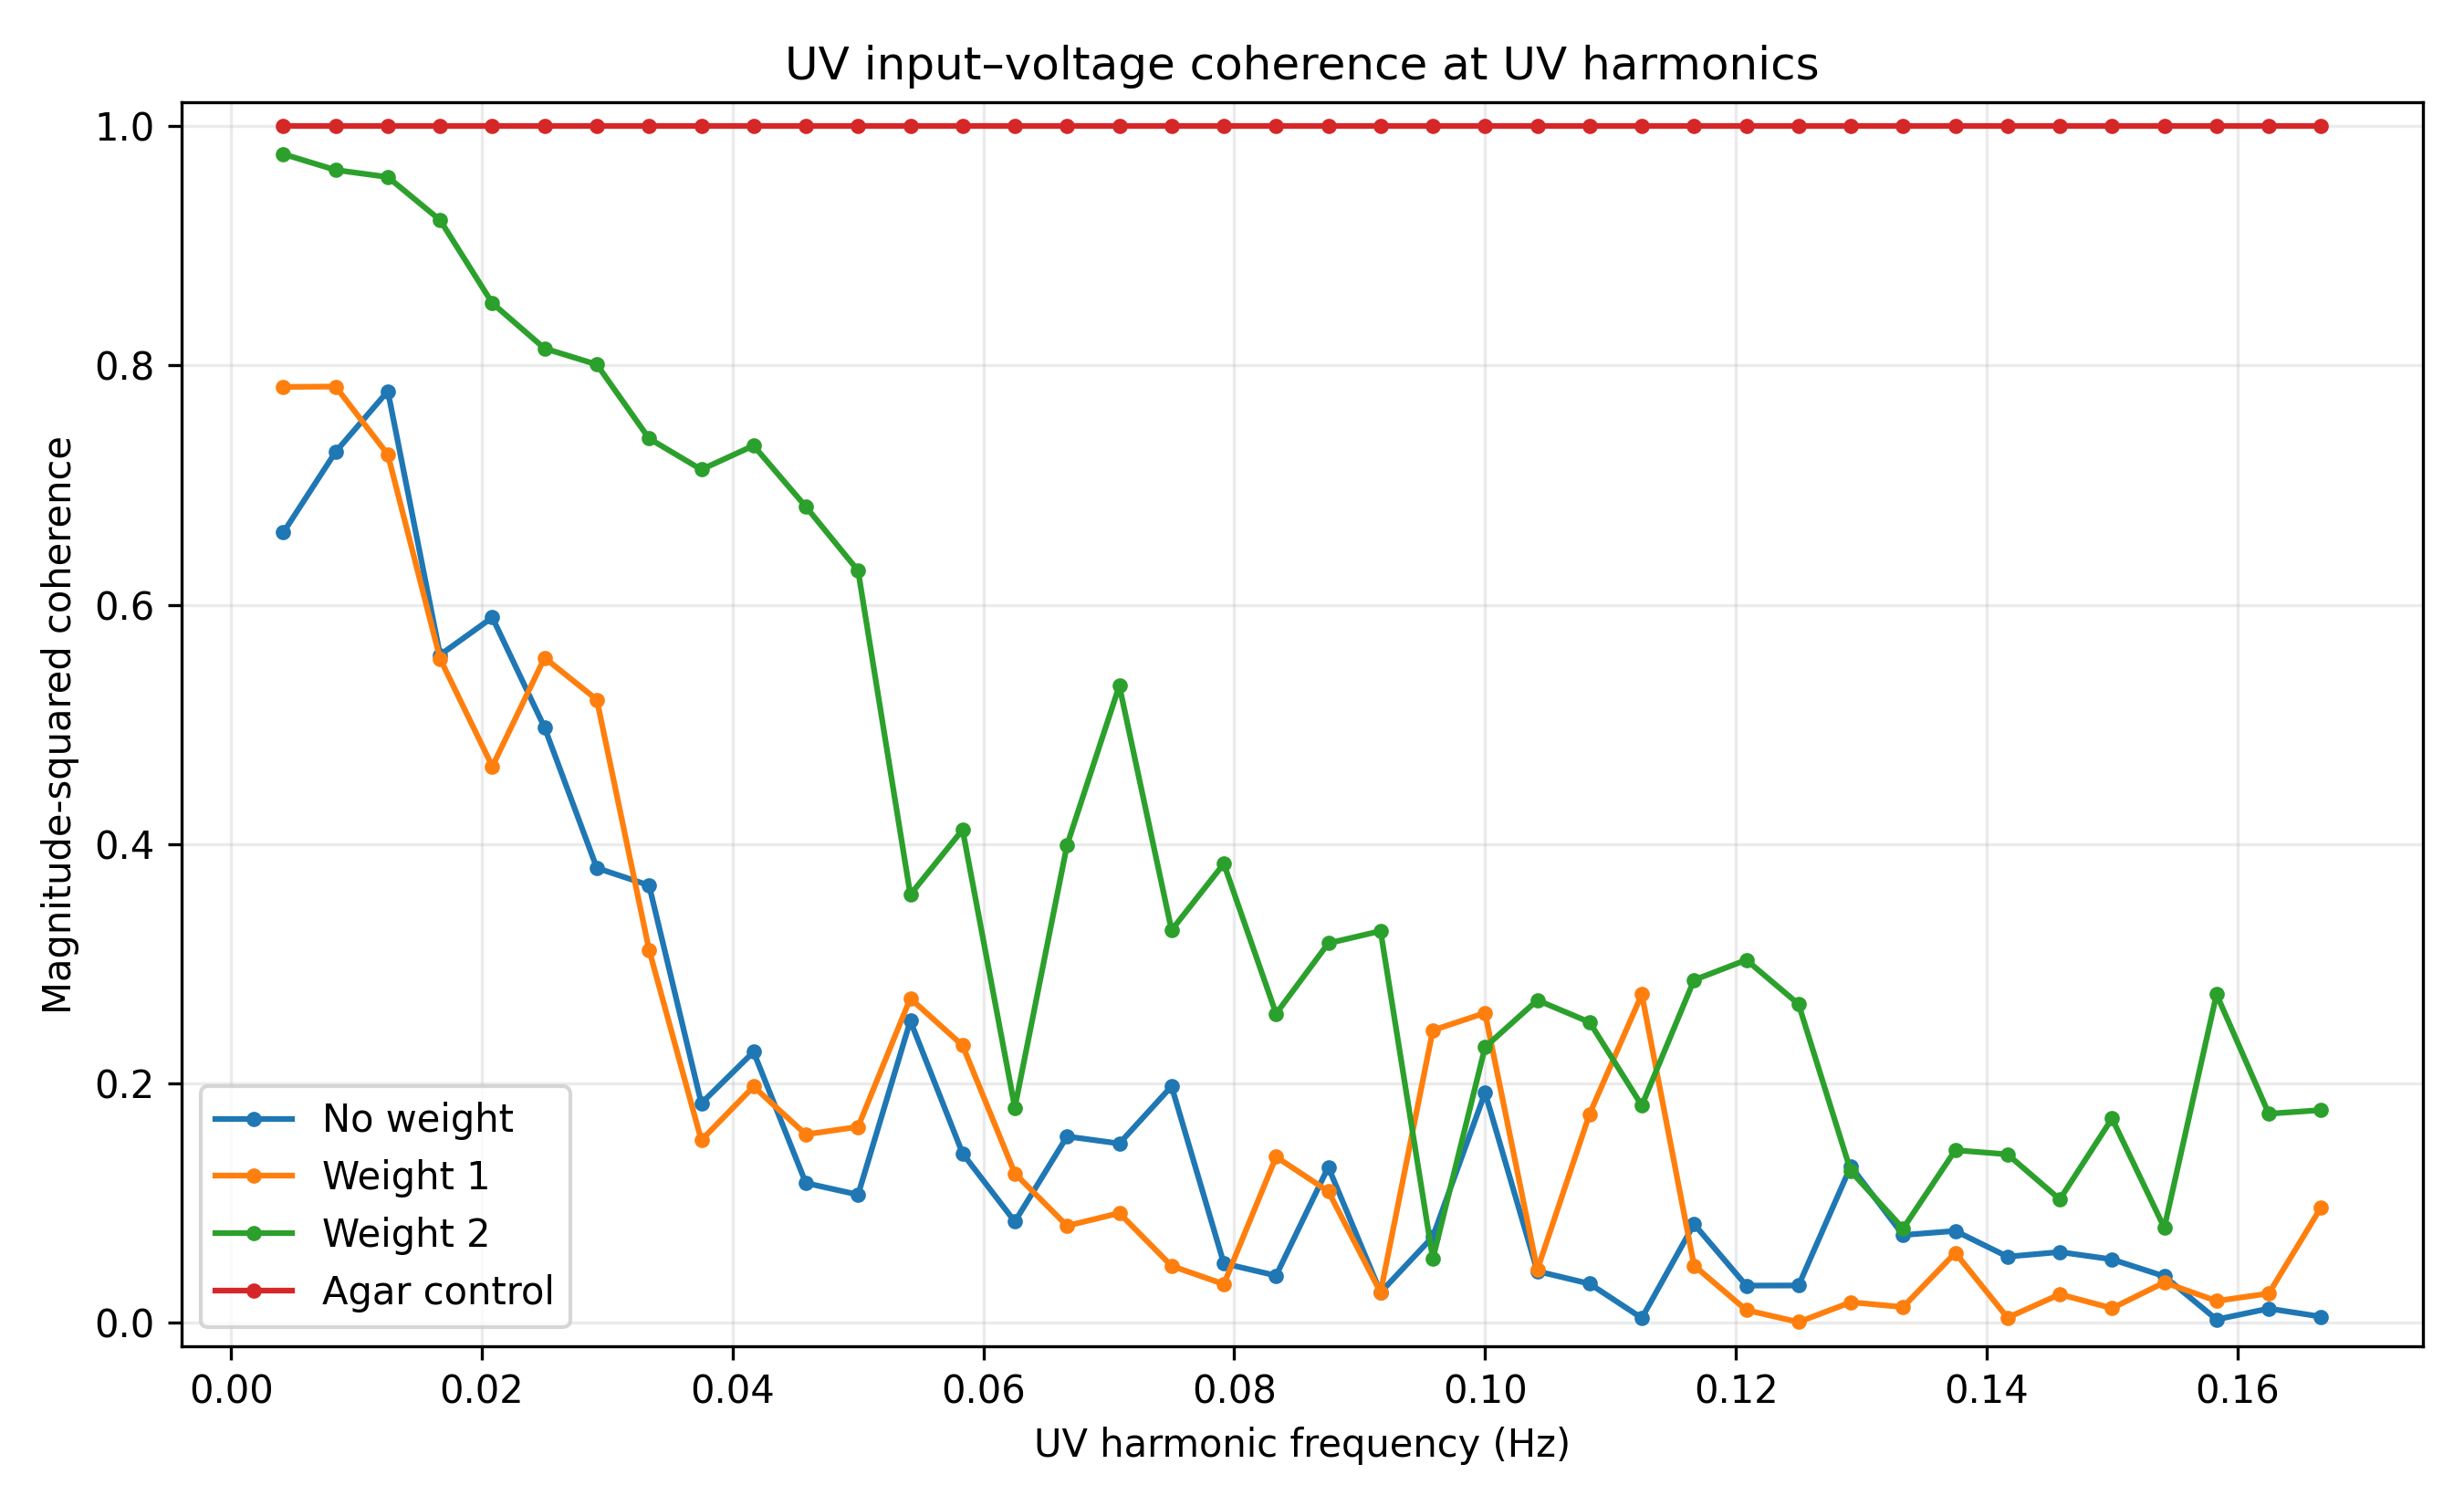
\includegraphics[width=0.92\textwidth]{figures/Figure_11_harmonic_coherence.png}
\caption{Magnitude-squared coherence between the reconstructed UV input and measured voltage at the UV harmonics.}\label{fig:harmonic_coherence}
\end{figure}

\subsection{Cycle-to-cycle evolution}

Harmonic gain was also evaluated separately for each UV cycle. This provides a frequency-domain counterpart to the cycle-by-cycle time-domain metrics and allows possible adaptation or evolution of the response to be identified.

\begin{figure}[H]\centering
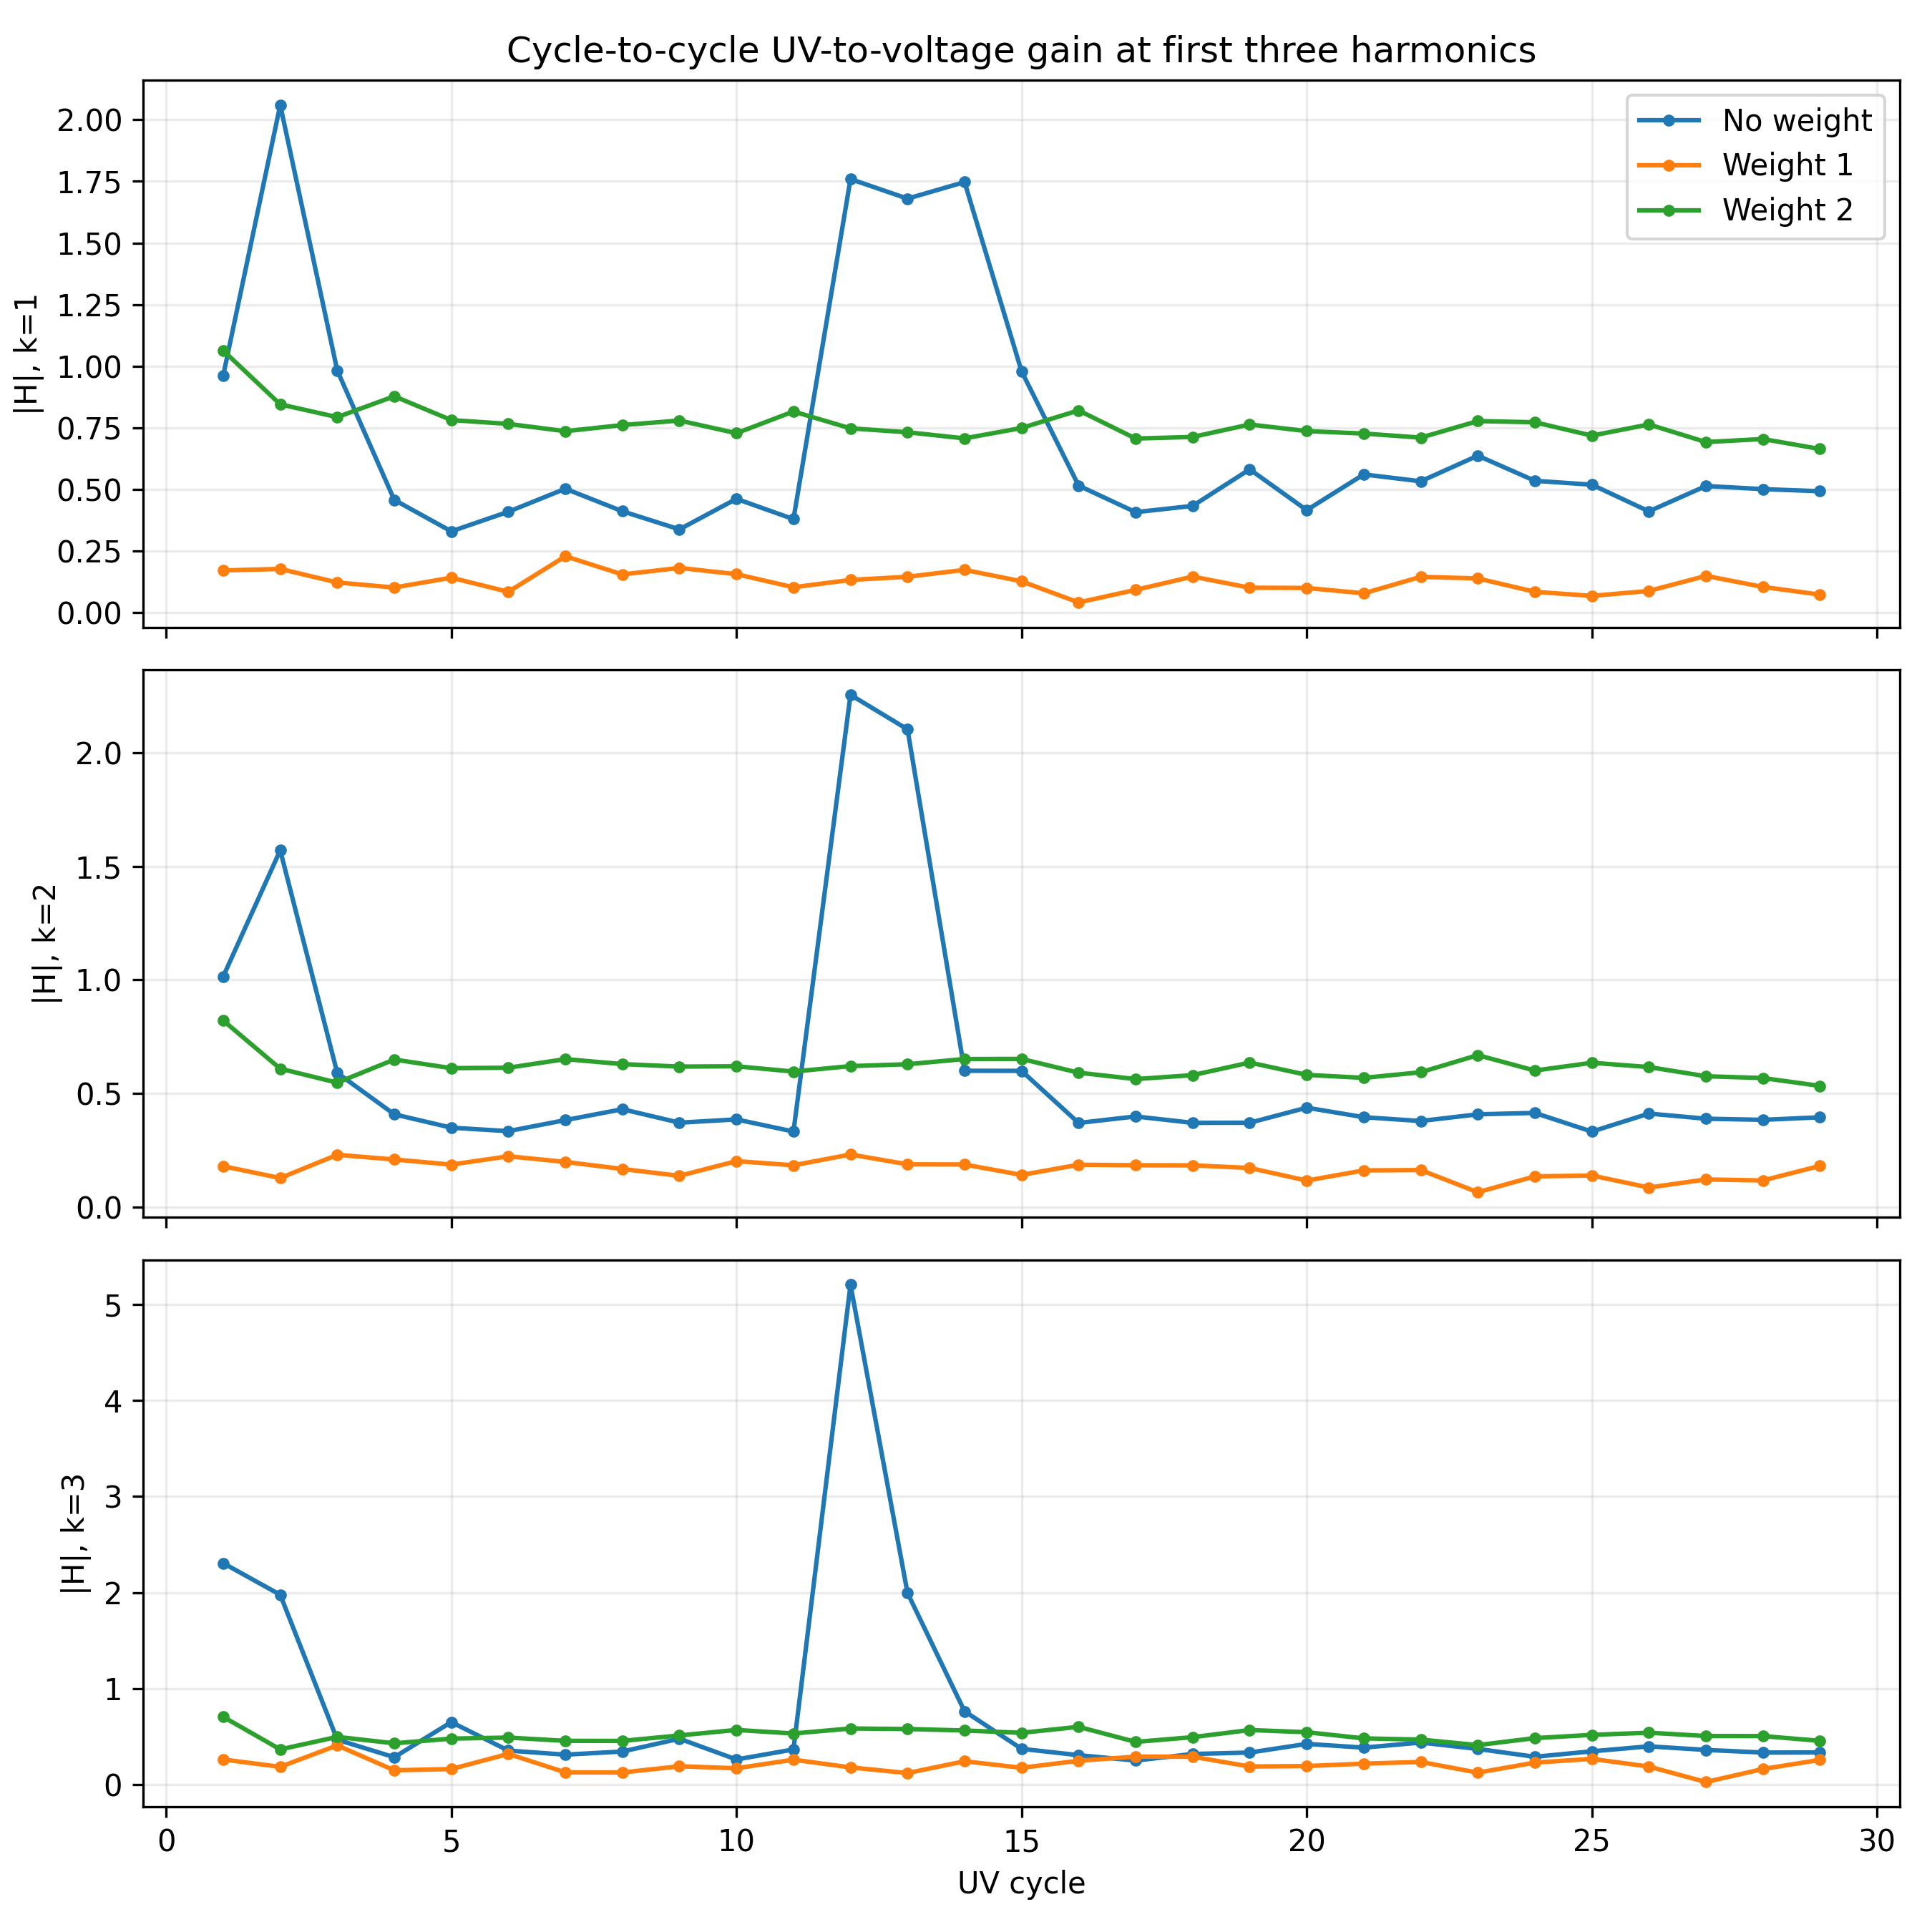
\includegraphics[width=0.92\textwidth]{figures/Figure_12_cycle_harmonic_gain.png}
\caption{Cycle-to-cycle harmonic gain for the first three UV harmonics.}\label{fig:cycle_harmonic_gain}
\end{figure}

\subsection{Unified stimulus--response description}

The two analyses can be viewed as complementary projections of the same experiment:
\[
\boxed{\text{UV input}\rightarrow\text{mycelium under mechanical state }L\rightarrow V(t)}.
\]
Time-domain observables are
\[
\{A_{\max},t_{50},t_{90},t_{\mathrm{rec}},\mathrm{AUC}\},
\]
while frequency-domain observables are
\[
\{|H_k|,\arg(H_k),C_k\}.
\]
For the current data, Weight 2 simultaneously shows the largest time-domain response amplitude, fastest apparent rise and recovery, largest UV AUC, largest fundamental harmonic gain, high coherence with the periodic UV input, and high phase consistency across repeated cycles. This convergence makes Weight 2 a particularly interesting pilot observation, but it remains a single biological run.

Recent fungal electrophysiology work has likewise used short-time Fourier analysis to extract frequency patterns from extracellular voltage recordings, supporting the methodological relevance of frequency-domain analysis while using a different experimental system and objective \cite{Buffi2025}.

\subsection{Next experimental test}

The next experiment should retain the present time-domain measurements while adding harmonic gain and UV--voltage coherence as predefined response descriptors. For each independent sample, several standardized UV cycles should be recorded. The independent experimental unit must remain the biological sample rather than the repeated cycle. With multiple independent samples, we can test whether mechanical loading is associated with reproducible changes in amplitude, kinetics, harmonic gain, and UV--voltage coherence.

The sharpened hypothesis is:
\[
\boxed{\text{Mechanical state modulates both the temporal kinetics and the frequency-domain coupling of mycelial electrical responses to UV stimulation.}}
\]

\section{Interpretation and limitations}

The current data support the following pilot observations:

\begin{enumerate}
    \item Repeated UV illumination produces a reproducible,
    time-dependent extracellular voltage response in the mycelium recordings.
    \item The response waveform differs between the three mycelium
    recordings. In particular, loaded replicate 2 exhibits a strong,
    predominantly positive and comparatively rapid response.
    \item The response amplitude in loaded replicate 2 decreases over the
    repeated UV sequence, suggesting adaptation of the measured response
    within that experiment.
    \item The agar control does not reproduce the characteristic positive
    mycelium response, although its short duration limits the strength of
    this comparison.
    \item The two recordings obtained with the same nominal static weight
    differ substantially. Therefore, the present data cannot by themselves
    establish a causal effect of static loading.
\end{enumerate}

The 30 UV cycles in a single recording are repeated observations within one
experimental run, not 30 independent biological samples. Consequently,
formal inference about the effect of static loading should be based on
multiple independent mycelium samples per loading condition.

\section{Reproducibility}

All numerical processing and figure generation are contained in
\texttt{mycelium\_analysis.py}. To reproduce the analysis:

\begin{verbatim}
python mycelium_analysis.py
\end{verbatim}

The script reads the four NumPy files from the \texttt{data/} directory and
writes figures to \texttt{figures/} and numerical results to
\texttt{results/}.

\section{Recommended next experimental step}

For a statistically defensible study of static loading, the independent
experimental unit should be the mycelium sample rather than the individual
UV cycle. A useful design would therefore include several independent
samples under zero load and several independent samples under the same
static load, with the repeated UV cycles retained as within-sample repeated
measurements.

\begin{thebibliography}{9}
\bibitem{Buffi2025}
M. Buffi et al., ``Detection of electrical signals in fungal mycelia in response to external stimuli,'' \emph{iScience}, vol. 28, no. 10, 113484, 2025. \doi{10.1016/j.isci.2025.113484}

\bibitem{Mishra2024}
A. K. Mishra, J. Kim, H. Baghdadi, B. R. Johnson, K. T. Hodge, and R. F. Shepherd,
``Sensorimotor control of robots mediated by electrophysiological measurements of fungal mycelia,''
\emph{Science Robotics}, vol. 9, no. 93, eadk8019, 2024.
\doi{10.1126/scirobotics.adk8019}
\end{thebibliography}

\end{document}
